% !TeX root = ../main.tex

\chapter{面向心理健康的大模型情感对话方法研究}

近年来,心理健康问题日益受到全球社会的广泛关注,抑郁症、焦虑症等心理障碍的患病率持续上升,尤其是在高压力环境下,人们的情绪管理与心理调适需求显著增加。传统的心理健康干预主要依赖于专业心理咨询师进行面对面的交流,但由于心理咨询资源有限、服务成本高昂以及社会对心理健康问题的认知偏差,使得大量有心理健康需求的个体难以获得及时的帮助。此外,现有的在线心理健康服务虽已发展出问卷测评、文本咨询、电话心理援助等方式,但仍存在交互方式单一、个性化不足、缺乏情感共鸣等问题,无法完全替代专业咨询。随着人工智能技术的迅速发展,基于自然语言处理(NLP)和大语言模型(LLM)的智能心理对话系统逐渐成为辅助心理健康对话支持的新方向,借助大模型的强大理解能力和生成能力,可以为用户提供更自然、更具共情能力的情感交互体验。

与传统的基于规则或浅层机器学习的情感对话系统不同,大模型(LLM) 具备大规模预训练能力,可以通过深度学习从海量数据中学习语言模式、心理学知识和情感表达方式,从而模拟人类心理咨询师的对话风格。然而,直接应用通用大模型进行心理健康对话仍面临诸多挑战,如情感理解不足、共情能力欠缺、心理健康知识偏差、生成内容的安全性和伦理合规性问题。因此本文设计了一个面向心理健康的情感对话大模型 PycoLLM,主要构建思路包括三个方向:(1)构建了一个高质量的心理健康对话数据集,以提高模型在心理场景下的适应能力;(2)二是通过有监督微调方法增强模型的心理咨询能力,使其具备更强的情感共鸣和问题应对能力;(3)为了评估估模型在心理健康对话任务中的综合表现,本文设计了一个心理学领域评估测试集,以衡量模型在不同心理咨询场景下的理解、推理和情感共鸣能力。

为了验证 PsycoLLM 的效果,本章在所构建的心理健康对话数据集上进行了训练,并在心理学评估测试集上进行了评估。实验结果表明,经过专用心理知识注入后训练的 PsycoLLM 在心理健康任务中取得了显著的性能提升,相较于基线模型,PsycoLLM 在心理学评估测集上多项评估指标上取得了更好的效果。此外,本章还对模型在心理健康对话任务中的应用进行了案例分析,展示了模型在实际心理咨询场景中的应用效果。

\section{任务目标}

本章旨在研究和构建面向心理健康的大模型情感对话方法,以提升人工智能在心理健康干预领域的应用能力。随着心理健康问题的日益严重,智能对话系统逐渐成为心理咨询和情感支持的重要工具。现有的情感对话系统在理解情绪、共情能力和心理健康知识的准确性方面仍存在较大挑战。

在情感对话任务中,早期的方法主要依赖于基于规则的系统和浅层机器学习模型(如 RNN、LSTM) 来进行情感识别与对话生成。这些小模型虽然在特定任务上取得了一定的效果,但由于建模能力有限、上下文理解不足、缺乏情感推理能力,在复杂心理对话场景中的应用效果受到了严重制约。例如,基于规则的方法依赖于手工制定的对话逻辑和关键词匹配,面对更开放的自然语言表达时,难以进行个性化情感识别和精准的心理干预。而 RNN、LSTM 等深度学习模型尽管可以通过训练数据学习情感模式,但由于其长程依赖弱、难以建模复杂的情感语境,导致在多轮对话中容易丢失关键的情感信息。此外,这类小模型的数据需求较大但泛化能力较差。

随着深度学习与大规模预训练语言模型(LLM)的兴起,通用大模型(如 GPT-4o、LLaMA、Qwen 等)展现出了强大的自然语言理解与生成能力,为心理健康对话系统提供了新的可能。然而,尽管这些通用大模型在对话生成上取得了显著进展,它们在心理健康任务上的表现仍然存在一定的局限性。首先,通用大模型缺乏专业化的心理学知识,虽然它们可以基于大规模互联网数据学习基本的情感表达,但由于其训练数据覆盖面广泛,导致其在心理咨询领域的专业性较弱,容易生成泛化性强但缺乏针对性的心理健康建议。其次,这些模型对心理健康对话中的情感理解仍然有限,在共情表达、情绪安抚、心理咨询逻辑推理等方面表现不够稳定。因此,仅依赖通用大模型进行心理健康对话任务无法满足实际应用中的需求,需要进一步结合心理学知识注入进一步提升模型的专业性。

基于上面的情况,本章聚焦于构建一个面向心理健康的情感对话大模型 PsycoLLM,旨在提升模型在心理咨询和情感支持任务中的性能。由于心理健康领域存在高质量数据稀缺的问题,因此本研究的第一个任务是构建一个覆盖广泛心理健康话题、具备共情表达能力的心理健康对话数据集作为模型的训练集,在该数据集基础上训练构建一个具备共情机制的心理健康大模型 PsycoLLM。

由于缺乏专门针对心理健康任务的标准化评测方法,为此,本文的第二个任务是构建心理健康对话模型的评测评估,以全面评估 PsycoLLM 在心理健康任务中的表现。该评测体系不仅包含 基于心理学领域的选择题测试(MCQ)、案例分析测试(Case-based Evaluation),以及自动化评测指标(如 ROUGE、BLEU、BERTScore),并为该心理健康和情感对话领域的大模型优化与评估提供依据和支持。

\section{具备共情机制的心理数据集构建}

本节详细介绍训练大模型所使用的数据集的构建过程。数据集主要包括单轮问答、多轮对话和知识性问答三类内容。数据集的构建流程如图~\ref{data-preparation}所示。

\begin{figure}[ht]
  \centering
  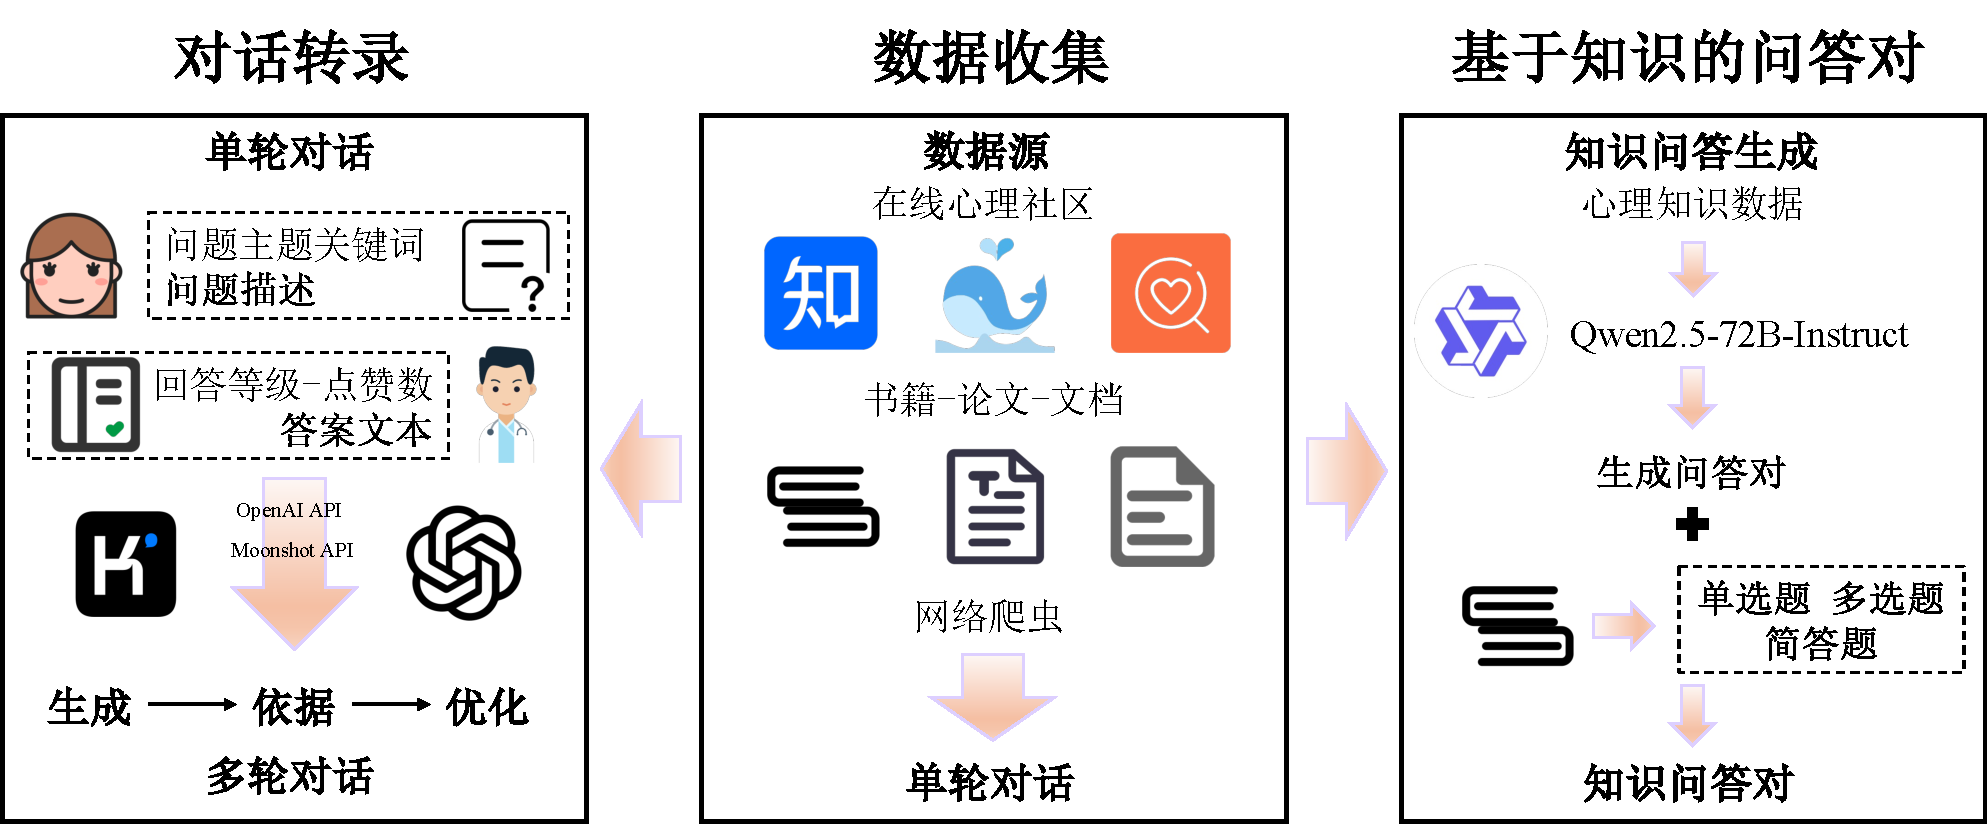
\includegraphics[width=1\textwidth]{data-preparation.pdf}
  \caption{数据集构建方法}
  \label{data-preparation}
\end{figure}

\subsection{单轮问答数据构建}

单轮对话问答数据集的构建旨在为模型提供高质量的心理健康问题与解决方案对,支持心理健康领域中的快速问题解答。为了构建这一数据集,本文从多个公开的心理学平台获取了大量真实的用户提问及其专业解答。这些平台包括壹心理(Yixinli)、知乎(Zhihu)等,这些网站致力于为寻求心理帮助的个体提供在线解答。用户在这些平台上通常会描述自己的心理困扰,并提出相关问题,随后,专业人士或有经验的个体会针对这些问题提供详细的解决方案或建议。本文从这些网站收集了超过267,000对问答数据。

在原始数据的收集过程中,用户提问通常会包含背景信息,并提出相关的心理健康问题。为了确保数据集的质量,本文对收集到的数据进行了多项重要的数据清洗处理,具体包括三个步骤:(1)去除无关内容,本文首先去除平台上出现的广告、推广信息等与核心数据无关的内容,这些无关内容会干扰数据的准确性,可能为模型训练引入噪声。(2)去除低质量回答,本文排除了用户点赞数低于5的回答,优先保留那些在用户中广泛认可的答案。点赞数可以作为用户对回答的认可度的一个衡量指标,较高的点赞数意味着该回答在公众中得到了较广泛的共识,能够反映出答案的有效性与可靠性。(3)去除低层次咨询师的回答,本文还排除了来自初级心理咨询师或个人回答者的回答,确保数据集反映出一定程度的专业意见。回答者的层次是其专业能力的一个重要指标,因此,仅保留有丰富经验的专业人士提供的回答,能够提高数据集的质量。

经过这些数据清洗步骤后,本文最终获得了超过155,000对单轮问答数据。这些数据涵盖了多个心理健康领域的问题和回答,能够为心理健康大模型提供广泛且具有代表性的信息。在数据处理后,本文对数据进行了详细的统计分析,主要从不同话题进行分类。本文将这些问答数据分为9个主要话题,具体的话题分布如图~\ref{topic-distribution}。从中可以观察到,情绪问题与调节、以及人际关系和社交问题占据了数据集的较大比例,每个话题均超过了总数据的20\%。其次,家庭与婚姻、个人成长与发展等话题也占据了较为重要的位置,各自占比超过10\%。这些话题的高频出现表明,情绪调节、人际关系等是人们在心理健康问题中最为关注的领域。

\begin{figure}[ht]
  \centering
  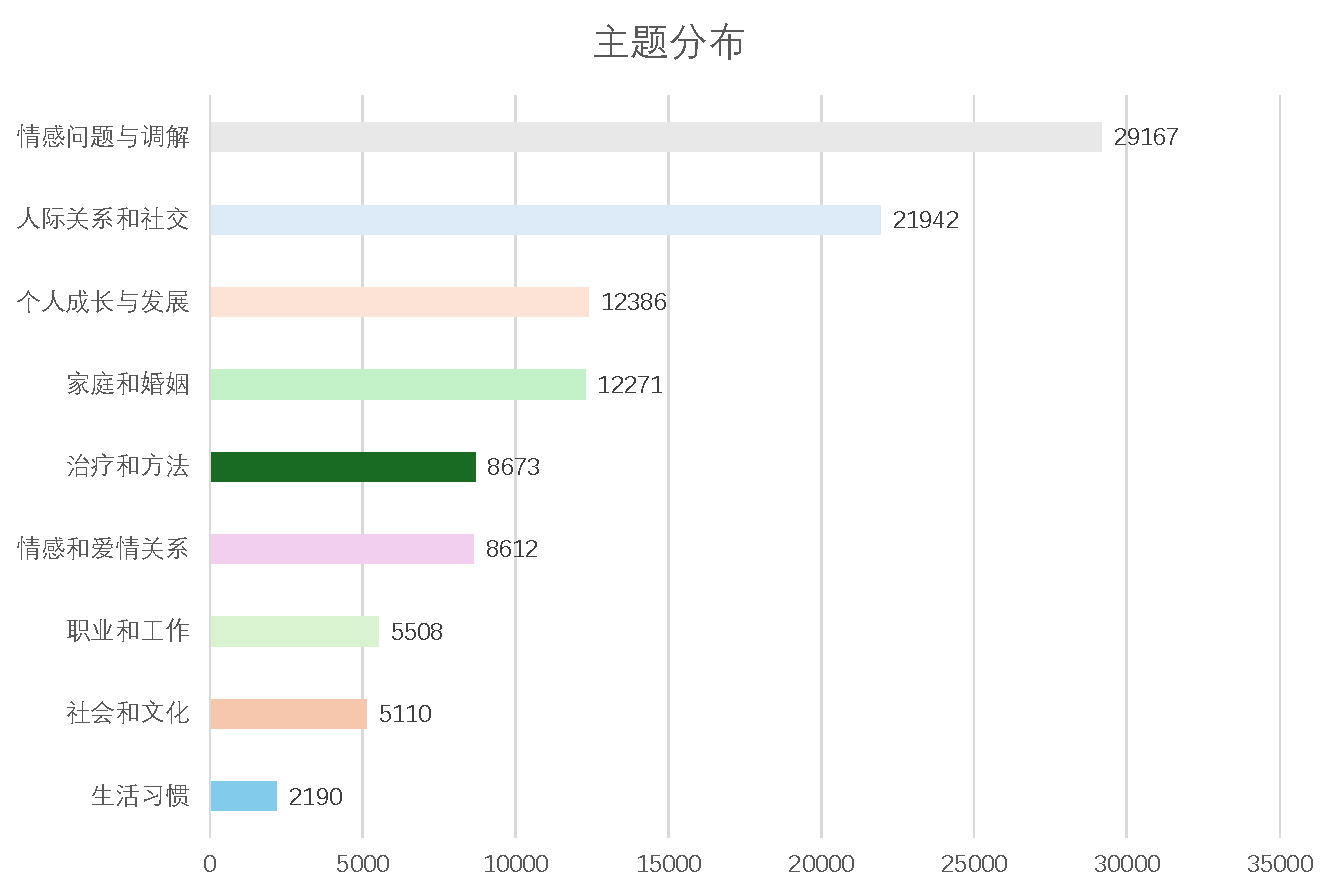
\includegraphics[width=1\textwidth]{topic-distribution.pdf}
  \caption{话题分布}
  \label{topic-distribution}
\end{figure}

此外,为了更直观地呈现数据的分布情况,本文通过词云的方式对收集的数据进行了可视化,如图 ~\ref{wordcloud} 所示。这种可视化方式展现了数据集中出现频率较高的关键词,进一步揭示了这些数据与日常心理咨询的密切联系。词云的展示不仅增强了对数据的理解,也表明这些数据反映了实际心理健康对话中的常见问题和需求,增强了数据的现实性和合理性。该单轮对话问答数据集为心理健康领域中的情绪分析与对话生成提供了高质量的基础数据。这一数据集的应用将有助于训练出能够处理实际心理咨询问题的大型语言模型,提升模型在心理健康服务中的效果和应用价值。

\begin{figure}[ht]
  \centering
  
\includegraphics[width=1\textwidth]{wordcloud.png}
  \caption{数据的词云展示}
  \label{wordcloud}
\end{figure}

\subsection{多轮对话数据构建}

在单轮对话问答数据集构建的基础上,本文进一步构建了多轮对话数据集。多轮对话数据集的目标是模拟心理咨询师与求助者之间的逐步对话过程,通过不断的提问和反馈,深入了解求助者的心理状态和需求,从而提供更加有效的帮助。为了实现这一目标,本文从前述单轮对话问答数据集中选取了每个问题下获得最多点赞的回答,并使用 GPT-4 和 KimiChat 生成多轮对话数据。这个过程模拟了心理咨询师的行为,通过多轮提问和回应,逐渐揭示求助者的心理状态和需求。

多轮对话数据集主要包含两种角色:求助者和心理专业人士。本文采用了一个三步数据生成管道,以保证生成的数据高质量和贴合实际心理咨询对话的流程。数据生成管道的三个步骤包括:(1)第一步,本文使用适当的提示语(prompt)来指导KimiChat根据已选择的问答对生成多轮对话数据。选定的问答对作为先验知识,帮助KimiChat构建多轮对话,增强生成数据与真实对话的相似性和可信度。通过引导模型生成基于真实场景的对话数据,本文期望能够保持对话的自然流畅性,并准确反映实际心理咨询中常见的问答模式。(2)第二步,本文引入额外的提示语来评估生成的多轮对话中的回答是否能够基于原始问答对的内容得到支持。如果大多数回答能够通过原始数据中的信息进行验证,则认为该对话数据更好地反映了现实心理咨询师的对话流程。相反,如果多数回答是由模型主导生成,且未能有效利用原始数据中的上下文信息,那么这些数据条目需要进一步处理。本文通过进一步增强提示语,提升模型对事实证据的整合能力,确保生成内容紧扣原始数据中的相关信息,并且不影响对话的流畅性。(3)第三步,为了进一步提升多轮对话数据的质量,本文加入了针对共情、支持性、指导性和安全性等方面的修订提示。通过这些修订,本文增强了对话中的情感支持性和专业性,确保生成的对话更加符合心理咨询中的伦理和标准要求。最终,本文还进行了人工校对,进一步确保数据的准确性和高质量。

用于多轮对话生成、依据支持识别和对话评估的提示词如 ~\ref{tab:prompt-template} 所示。通过这三步法生成了符合实际心理咨询对话流程的数据。本文还对使用单一复杂提示语与三步法进行对比,发现单一提示语生成的数据往往缺乏信息整合,容易出现模板化的回答,而三步法能够更加全面地整合提供的事实信息,生成更符合实际对话流程的内容。因此,本文选择了采用三步管道方法来生成多轮对话数据。一个例子如图 ~\ref{fig:multi-dialog-generation} 所示,有三个步骤来生成高质量的数据。生成的多轮对话数据集具有较高的质量和实用性,能够为多轮对话中的情绪分析、共情表达等方面提供丰富的训练素材。最终的数据统计结果如表 ~\ref{tab:multi-dialog-statistics} 所示,展示了数据集的规模和各个话题的分布情况,进一步验证了本文生成的多轮对话数据的多样性和有效性。通过这一数据集构建过程,本文不仅提供了心理健康领域中多轮对话的典型样本,也为多轮对话生成与情绪分析任务的模型训练提供了高质量的支持。

\begin{table*}[t]
  \centering
  \caption{用于多轮对话生成、依据支持和对话评估的提示词}
  \label{tab:prompt-template}
  \resizebox{1\textwidth}{!}{
    \begin{tabular}{l|l}
      \toprule[1pt]
      提示词类别 & 提示词模版 \\
      \midrule
      多轮对话生成 &
      \begin{tabular}[c]{@{}l@{}}您是一位专家,深入研究了无数心理健康患者与医生之间的对话。\\
        请构建一段由求助者与心理医生进行的多轮连续对话记录。\\
        您将看到一个由用户提问和心理助手回答组成的问答形式。\\
        输出格式如下:\\
        用户:患者的陈述。\\
        心理助手:医生的安慰、建议和指导。\\
        用户:\dots \\
        心理助手:\dots \\
        对话应包括更多轮次的交流内容。
      \end{tabular}
      \\ \hline
      依据支持 &
      \begin{tabular}[c]{@{}l@{}}您是一位专业心理学家,曾提供过众多心理咨询服务。\\
        您的任务是从多轮对话问答中,识别心理医生每条回复的依据来源。\\
        请为多轮对话中的每一句回复,标明其依据来源,依据需从原始问答中提取。\\
        如果没有对应的依据来源,请直接输出“无对应来源”。\\
        输出格式如下:\\
        多轮对话中的回复:<原始对话>\\
        来源:<来自访客的自述/来自医生的回复/无对应来源>:<对应的原始文本>
      \end{tabular}
      \\ \hline
      对话评估 &
      \begin{tabular}[c]{@{}l@{}}您是一位心理学教授,精通心理学与语言学。\\
        从心理学教授的角度出发,请基于以下四个指标进行严格评判:\\
        1. 共情:心理医生是否能够真正理解访客的情绪和需求,并表达出真诚的关怀。\\
        2. 支持性:心理医生是否通过言语反馈表现出倾听访客的态度。\\
        3. 引导性:心理医生是否通过提问或提供选择,引导访客思考或行动。\\
        4. 安全性:心理医生的言语或行为是否可能对访客产生负面影响。
      \end{tabular}
      \\
      \bottomrule
    \end{tabular}
  }
\end{table*}


\begin{figure}[ht]
  \centering
  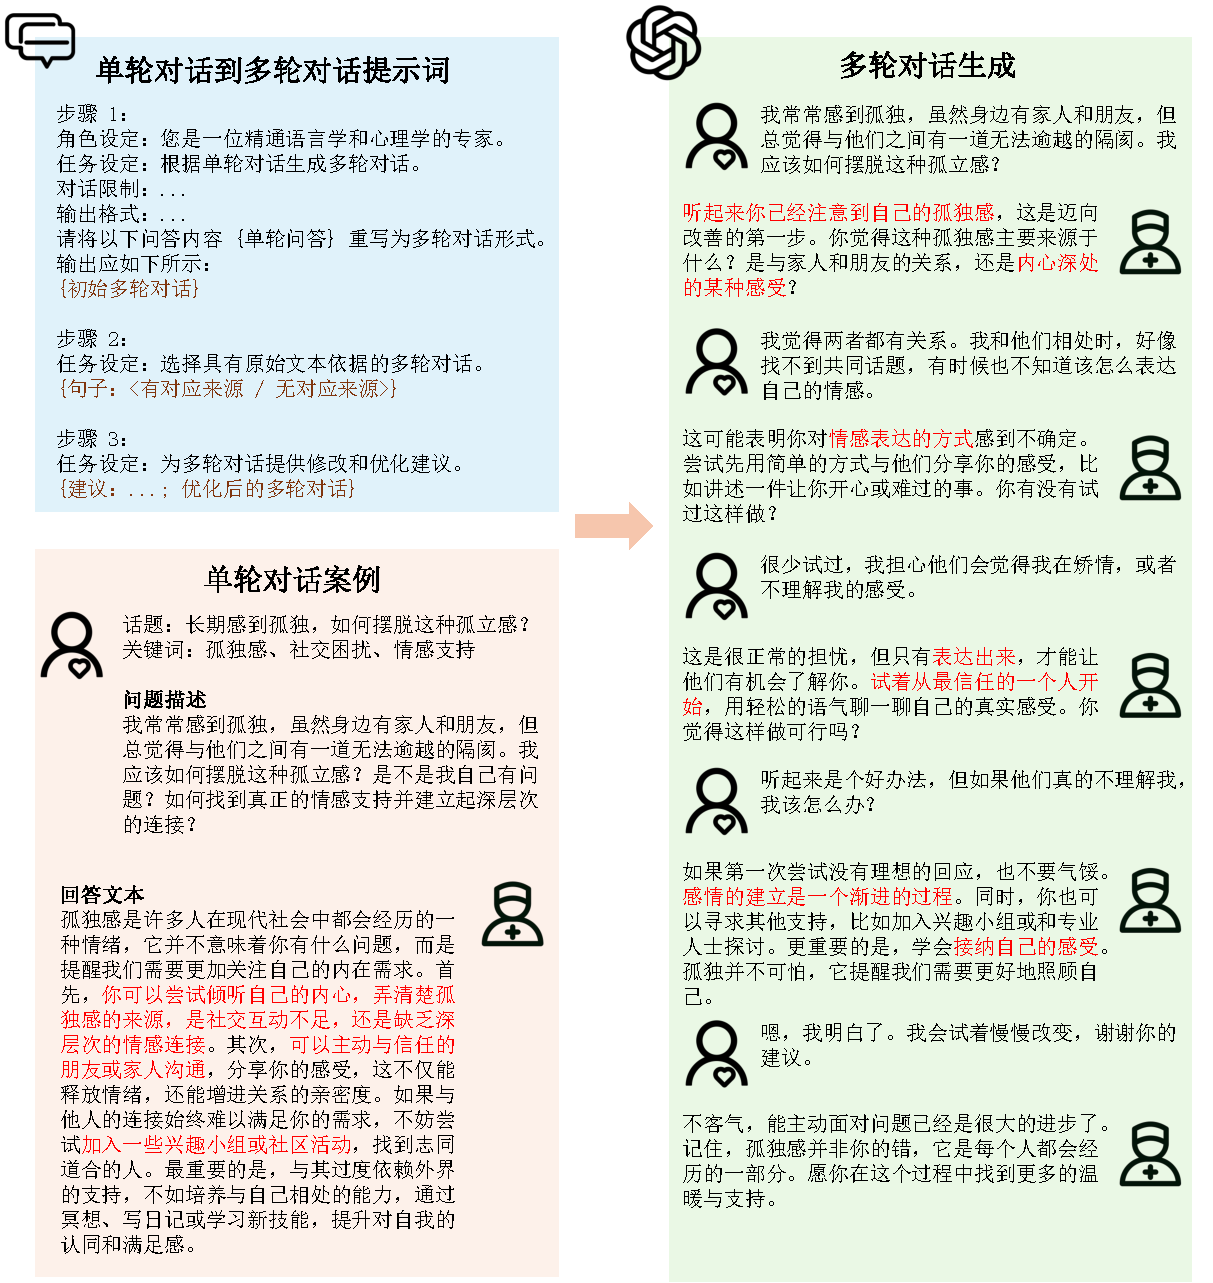
\includegraphics[width=1\textwidth]{multi-dialog-generation.pdf}
  \caption{生成的多轮对话数据示例}
  \label{fig:multi-dialog-generation}
\end{figure}

\begin{table}
  \centering
  \caption{多轮对话生成的数据统计}
  \label{tab:multi-dialog-statistics}
  \begin{tabular}{ll}
    \toprule
    统计类别 & 数据量 \\
    \midrule
    多轮对话数量 & 11511 \\
    平均对话轮数 & 5.90 \\
    每轮对话平均 Token 数 & 136.28 \\
    每轮对话平均问题 Token 数 & 43.62 \\
    每轮对话平均回答 Token 数 & 92.66 \\
    \bottomrule
  \end{tabular}
\end{table}

\subsection{知识性问答数据构建}

为了进一步丰富心理健康领域的数据集,本文引入了更具抽象性的心理学知识数据,包括对心理学术语的解释和相关理论的阐述。这些知识性问答数据不仅能提供日常交互的支持,还能为心理健康领域的深层次知识传递提供帮助。为了构建这一类基于知识的问答数据集,本文从网络上爬取了多本与心理学相关的书籍,并通过 Qwen2.5-72B-Instruct 模型从这些书籍中提取出知识型问答数据。具体而言,本文首先对书籍内容进行分段处理,使用预定义的固定长度将文本划分为若干段落,并根据距离最近的句子或段落作为分段标志。这些文本段落成为后续生成问答对的基本单位。接下来,本文利用大型语言模型(LLM)生成基于这些文本段落的问答对。生成的问答对中包括问题及其对应的答案,它们将作为后续处理的基础数据。

为了提高生成问答的质量和准确性,本文采用了双模块生成与评估方法:(1)学生模块:本文构建了两个基于LLM的学生模块,一个使用检索增强生成(RAG)技术,另一个则不使用RAG。两个模块分别生成各自的答案,并输出两个不同的答案集合。(2)教师模块:为了选择最佳答案,本文使用了一个基于LLM的教师模块,对来自学生模块的多个答案进行评估,并选择最优答案。这一过程能够确保生成的答案在内容的准确性和相关性方面得到保证,从而提高了问答数据的整体质量。

为了进一步确保生成的知识型问答数据的质量,本文还加入了人工验证环节。在这一环节中,人工评审人员会对生成的问答数据进行审核,剔除那些质量较低的问答对。人工验证的步骤对于确保数据集的准确性和实用性起到了关键作用。此外,本文还从多本心理学教材中提取了课后练习题及其解答分析,这些数据进一步丰富了本文基于知识的问答数据集。最终,通过这一系列处理流程,本文成功构建了一个包含约10000对知识型问答的高质量数据集。

这些基于知识的问答数据主要涉及心理学的基本概念、理论解释、治疗方法等内容,能够为心理健康模型提供系统性的理论支持。这类数据集不仅为心理学领域的研究人员提供了丰富的知识储备,也为模型训练提供了更加严谨和具有深度的知识性内容。综上所述,基于知识的问答数据集为心理健康领域提供了重要的理论支持,能够辅助模型进行更为精准的知识检索与应用分析。这一数据集的构建不仅拓宽了本文对心理健康领域知识的理解,也推动了心理健康大模型在理论层面和应用层面的深度发展。

\section{具备共情机制的心理大模型}

基于构建的心理健康数据,本文进一步训练出了具备共情机制的心理大模型 PsycoLLM,具备强大的情感文本理解和生成能力,PsycoLLM 整体系统架构如图 ~\ref{fig:work1-architecture} 所示。前述小节详细介绍了数据集的构建过程,本节将详细介绍基于基于 Transformer Decoder 架构的开源大模型的整体结构和训练部署过程。

\begin{figure}[ht]
  \centering
  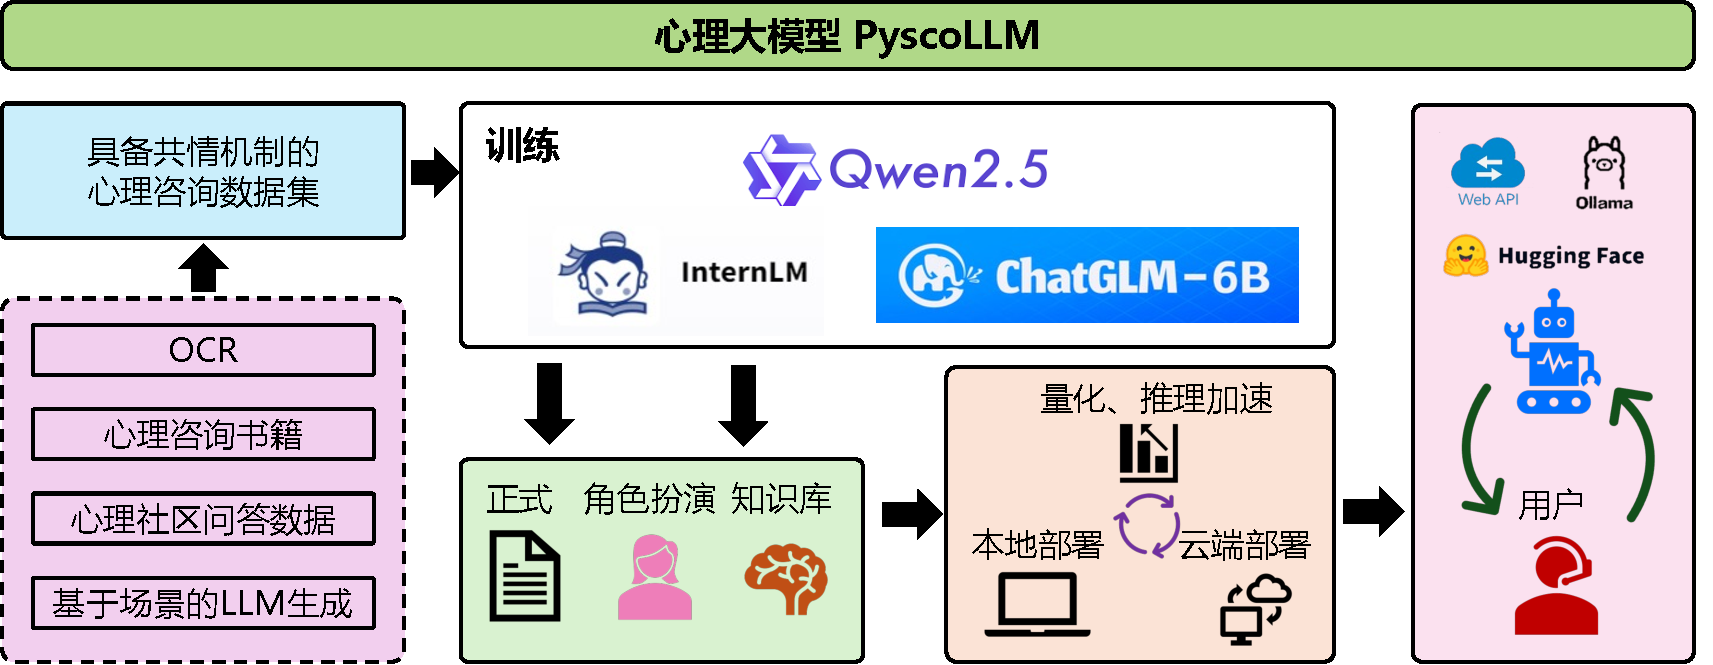
\includegraphics[width=1\textwidth]{work1-architecture.pdf}
  \caption{具备共情机制的心理大模型系统架构}
  \label{fig:work1-architecture}
\end{figure}

\subsection{模型整体结构}

从图 ~\ref{fig:Qwen-model} 可以看到,心理大模型的模型结构部分主要是基于中文领域的开源 Decoder 架构的大模型,包括 Qwen、InternLM、ChatGLM 等系列模型。以 Qwen2.5 模型为例,模型结构上采用了仅解码(Decoder-only)的Transformer架构,具备强大的文本理解和生成能力,能够对输入文本进行高效的特征编码与预测。整个模型的处理流程包括分词器、解码器和输出采样三个主要模块,下面对各模块的处理过程进行详细介绍。

\textbf{1. 分词器模块}

输入的原始文本首先经过分词器(Tokenizer)进行预处理,将连续的自然语言文本转换为模型可处理的子词单元(tokens)。Qwen 模型的tokenizer采用字节对编码(Byte Pair Encoding, BPE)算法。这一算法通过迭代地合并高频字符和子词对,将文本映射为更小的离散单元,从而有效地平衡了词汇表的大小和分词的粒度。分词过程:(1)初始化词汇表,本文将所有字符和子词对作为初始词汇表,每个字符和子词对作为一个独立的 token;(2)统计频率,统计文本中所有字符和子词对的频率,计算每个字符和子词对的出现次数;(3)合并频率最高的字符和子词对,选择频率最高的字符和子词对,将其合并为一个新的子词对,并更新词汇表;(4)重复步骤(2)和(3),迭代地统计频率和合并字符和子词对,直至达到预设的词汇表大小。

\textbf{2. 解码器模块}

经过分词器处理后的子词单元被编码为向量表示,随后进入模型的解码器(Decoder)进行特征建模和上下文学习。Qwen 的解码器在 Transformer 架构的基础上进行了优化,主要引入了以下核心技术:RMSNorm、RoPE、GQA、SwiGLU,从而提高了模型在长文本处理和高效推理方面的性能。

(1)RMSNorm 归一化层

RMSNorm(Root Mean Square Layer Normalization)\cite{Zhang_Sennrich_2019} 是一种归一化方法,作为 LayerNorm\cite{Ba_Kiros_Hinton_2016} 的改进版本,简化了计算流程,同时在性能上表现出色。与 LayerNorm 的主要区别是,RMSNorm 不进行均值归零,而是通过均方根(RMS)值进行归一化操作。设输入为 $x \in \mathbb{R}^d$,表示一个 $d$ 维向量,归一化过程为:
\begin{equation}
  \text{RMSNorm}(x) = \frac{x}{\text{RMS}(x)} \cdot \gamma,
\end{equation}
\begin{equation}
  \text{RMS}(x) = \sqrt{\frac{1}{d} \sum_{i=1}^d x_i^2},
\end{equation}
其中,$\gamma \in \mathbb{R}^d$ 是可学习的缩放参数。

(2)旋转位置编码

旋转位置编码(RoPE, Rotary Positional Embedding)\cite{Su_Lu_Pan_Wen_Liu_2021} 通过将位置编码与输入向量中的特征维度进行旋转变换,使模型能够捕捉相对位置信息,而不仅仅依赖于绝对位置。这种方法具有的优势包括:能够有效处理长序列文本,增强模型对长距离依赖的建模能力;通过旋转操作保持编码的可微性,有助于在自注意力机制中进行高效计算。在RoPE机制下,位置编码直接作用于特征向量的每个维度,从而使注意力计算能够自然地适应不同位置的相对关系。

\begin{figure}[ht]
  \centering
  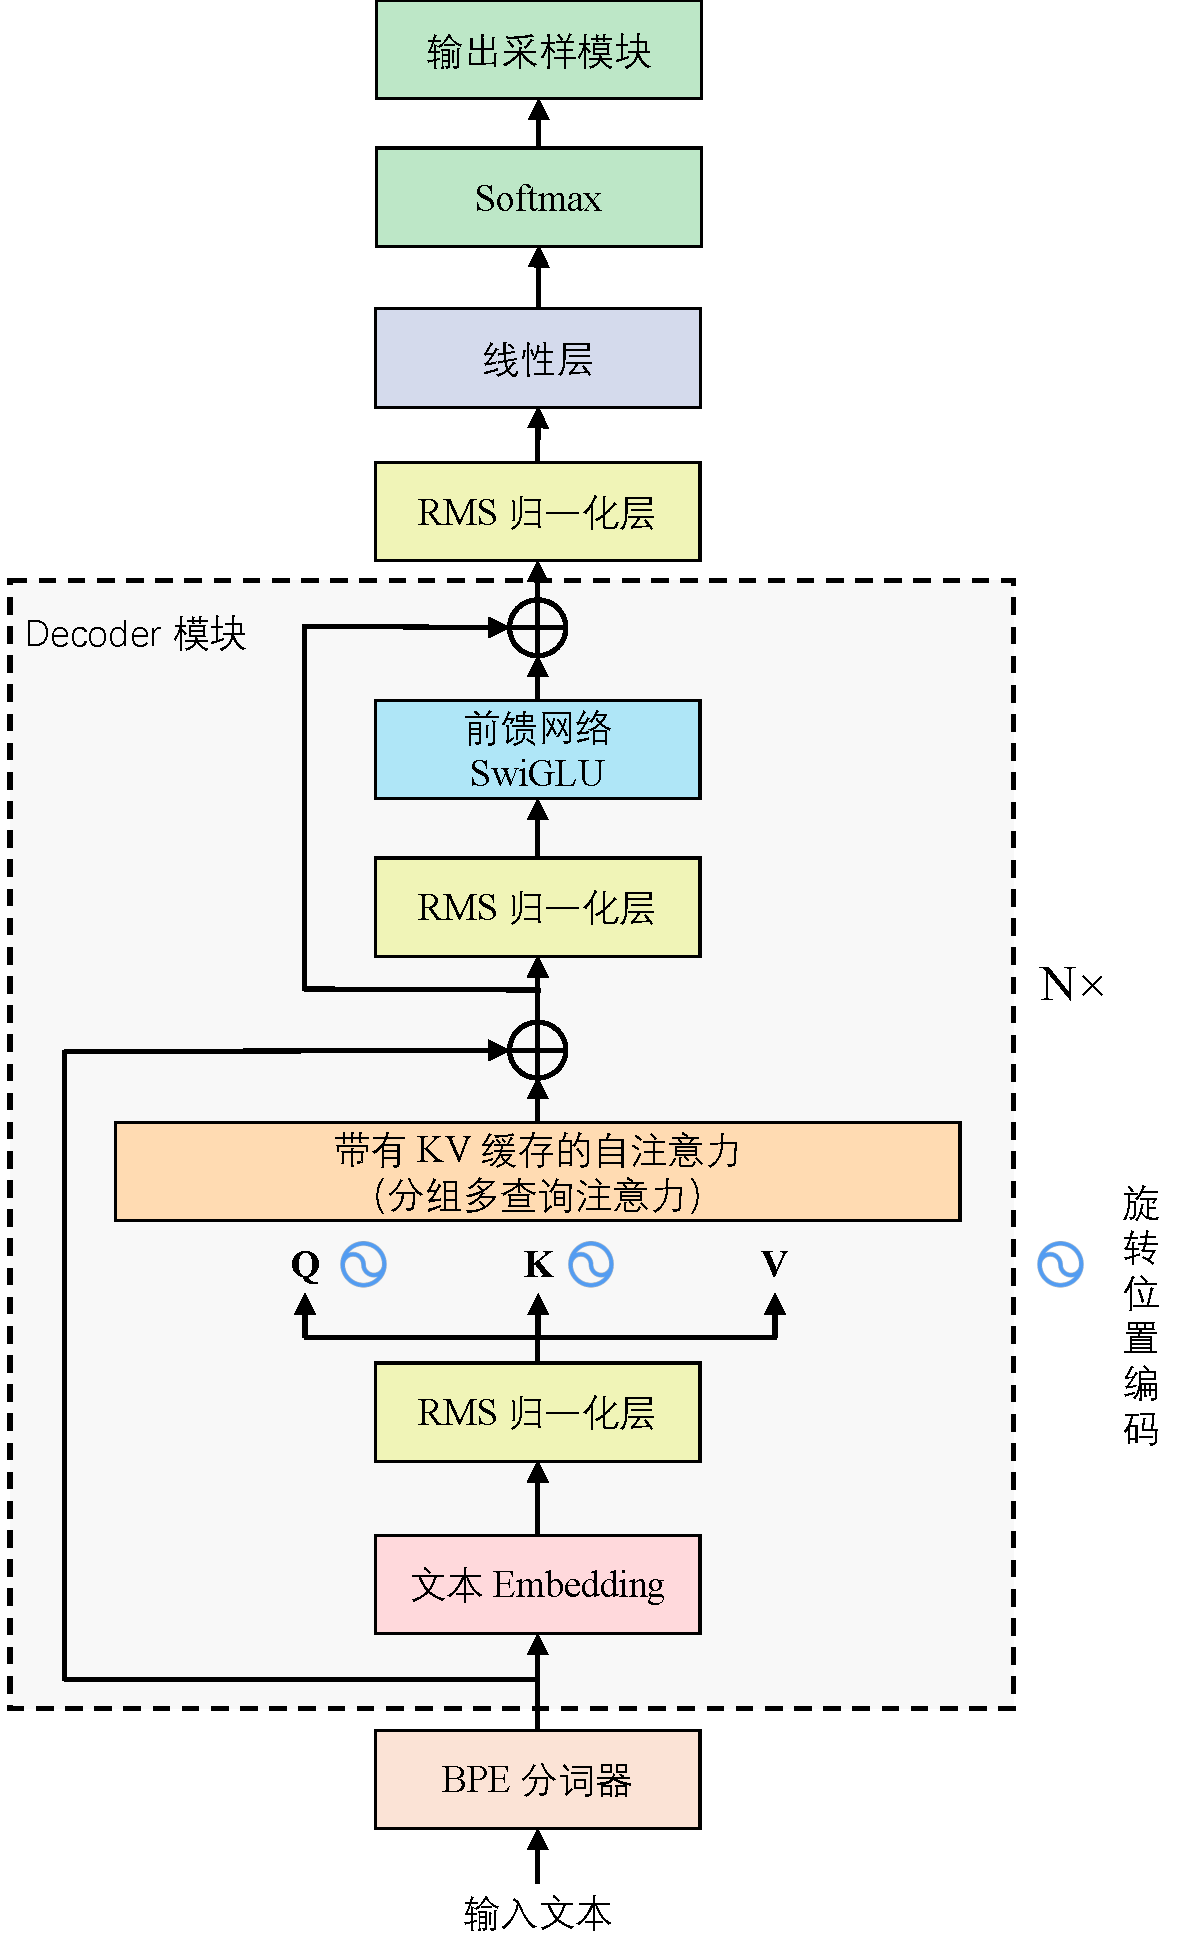
\includegraphics[width=0.5\textwidth]{Qwen-model.pdf}
  \caption{模型结构图}
  \label{fig:Qwen-model}
\end{figure}

(3)分组多查询注意力

分组查询注意力(GQA, Grouped Multi-Query Attention)\cite{ainslie2023gqatraininggeneralizedmultiquery} 对传统的自注意力机制进行了优化,减少了计算复杂度,尤其在大模型推理过程中体现出显著优势。其核心思想包括:将查询向量(Query)分组,每组共享一个注意力权重,从而减少查询与键(Key)之间的计算量;在保持注意力效果的同时,显著降低了计算开销和显存消耗,提升了推理效率。GQA机制的引入使Qwen2能够在处理长文本任务时更加高效,适合大规模部署和实际应用。

(4)SwiGLU 激活函数

Qwen 采用了 SwiGLU\cite{Shazeer_2020} 作为激活函数,这是一种基于GLU(Gated Linear Unit)的改进版本。SwiGLU通过以下公式进行计算:
\begin{equation}
  \text{SwiGLU}(x) = \text{Swish}(x) \cdot W_2 ( \text{GELU}(W_1 x) ),
\end{equation}
其中,$\text{Swish}(x) = x \cdot \text{sigmoid}(x)$。SwiGLU的优势包括:在保留GLU门控机制的前提下,通过Swish函数引入平滑非线性特征,增强模型表达能力;提高了训练的稳定性和效果,使模型在复杂任务中能够更好地收敛。

\textbf{3. 输出采样模块}

经过解码器处理后,最终输出的特征表示将通过一个线性层映射到词汇表的维度,并通过Softmax函数计算各个token的概率分布。具体过程包括三个步骤:(1)线性变换,将隐藏状态映射为与词汇表大小相同的向量;(2)概率分布,通过Softmax函数计算每个词汇的生成概率;(3)输出结果,选择概率最大的 token,或根据采样策略(如温度采样)生成最终的输出文本。输出采样模块实现了从隐藏表示到自然语言输出的转换,使模型能够根据输入文本生成符合语义逻辑的高质量文本。

\vspace{1em}

综上所述,模型通过分词器模块将输入文本编码为子词单元,利用优化后的解码器模块(结合RMSNorm、RoPE、GQA和SwiGLU技术)进行特征建模,最终通过输出采样模块生成文本输出。这一整体结构不仅保证了模型对输入信息的高效处理,还提升了对长序列和复杂情绪信息的建模能力,为所开发的大模型在心理健康领域的应用提供了强大的技术支持。

\subsection{有监督微调方法}

在获取高质量的心理学数据集后,本文进一步采用有监督微调(Supervised Fine-Tuning,SFT)技术,对大型语言模型进行定向优化,以增强模型在心理学领域的能力。本文选择 Qwen2.5-14B-Instruct 作为底座基础模型,开发本节的心理大模型。

在训练阶段,输入文本被表示为一个序列 $x = \{x_1, x_2, ..., x_L\}$,其中 $x_i$ 为文本中的一个标记(token),$L$ 是文本序列的长度。Qwen模型的核心架构基于Transformer解码器结构,它是一种典型的自回归框架,旨在按顺序预测文本序列中的每一个词。这一预测过程可以通过以下数学公式进行描述:
\begin{equation}
  p(x) = \prod_{t=1}^{L} p(x_t \mid x_1, ..., x_{t-1}).
\end{equation}
在训练时,本文采用交叉熵损失函数作为目标函数。模型的训练目标是最大化给定输入数据下的预测序列的负条件对数似然。具体而言,参数优化的目标可以表示为:
\begin{equation}
  \theta^* = \arg \max_{\theta} \sum_{t=1}^{L} \log p(x_t \mid x_1, ..., x_{t-1}; \theta),
\end{equation}
其中,$\theta$ 为模型的可训练参数。通过上述有监督微调过程,模型不仅继承了基础模型在自然语言处理中的强大性能,还通过高质量心理学数据的定向训练,进一步提升了模型在心理健康场景下的情绪理解、共情对话及专业知识问答等方面的能力。这一训练技术为构建心理健康领域的大模型提供了有效的方法与实践支持。

\subsection{LoRA 微调方法}

\begin{figure}[ht]
  \centering
  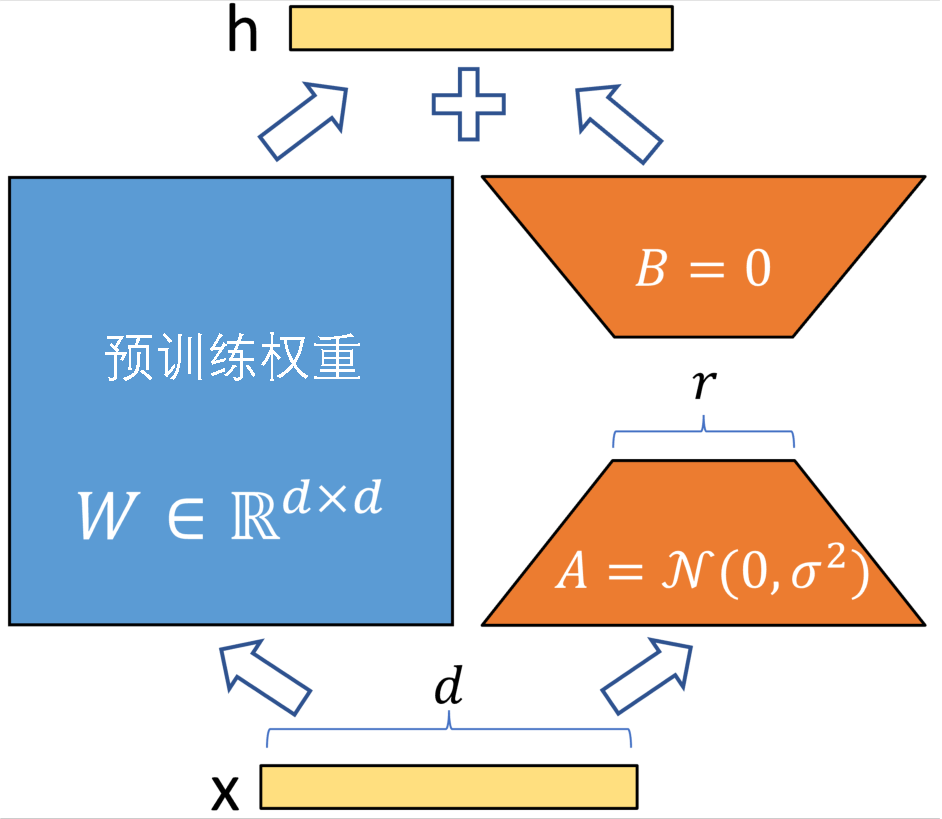
\includegraphics[width=0.5\textwidth]{LoRA.pdf}
  \caption{LoRA 微调方法}
  \label{fig:LoRA}
\end{figure}

为了进一步优化训练过程并提高计算效率,本文采用了 LoRA(Low-Rank Adaptation)\cite{hu2022lora} 技术对模型进行微调。如图 ~\ref{fig:LoRA} 所示,LoRA 技术通过学习一个小参数的低秩矩阵来近似模型权重矩阵 W 的更新。在训练过程中,仅优化这些低秩矩阵的参数,而不对整个权重矩阵进行更新。具体来说,这种方法利用了权重矩阵的低秩分解,将大规模参数的训练需求降低到一个更小的低秩空间,从而有效减少了计算资源的消耗,同时保留了模型的性能。

在本研究中,LoRA 微调技术的使用带来了显著的性能提升,使得模型在心理健康领域的情绪识别任务中表现更加精准且高效。这种微调方法不仅降低了训练成本,还确保了模型能够在大规模数据上进行有效学习,从而更好地支持实际应用中的情绪分析和心理对话支持系统。

\subsection{大模型推理部署}

本章主要介绍具备共情机制的心理大模型 PsycoLLM 在推理阶段的部署方案。随着大规模语言模型(LLM)在心理健康领域的应用不断深入,需要保证推理速度和资源利用效率的同时,提供高质量的情感理解和生成能力。为了满足不同场景的需求,本章探讨了远程服务部署和本地化部署两种策略,并详细介绍了 vLLM\cite{kwon2023efficient}、SGLang\cite{zheng2024SGLangefficientexecutionstructured} 以及 Ollama 等优化技术在 PsycoLLM 部署中的应用。

\textbf{1. 远程服务部署}

在实际应用中,大规模语言模型通常采用云端 GPU 推理架构,以满足高并发访问需求,同时降低终端设备的计算压力。PsycoLLM 的推理服务基于 vLLM 和 SGLang 技术,提供高效、低延迟的文本生成能力。这些技术主要优化了推理过程中计算资源的利用方式,使得 PsycoLLM 能够在心理健康应用场景下提供流畅的对话体验。

(1)vLLM:与传统推理方法相比,vLLM 采用了分页注意力机制(PagedAttention) 机制,大幅度提升了推理速度和 GPU 内存利用率。在传统推理过程中,每次生成新 token 时,模型需要计算所有前序 token 的注意力(attention),这导致了计算冗余和显存开销较大的问题。而 PagedAttention 通过动态缓存的方式,仅存储模型推理过程中的有效键值对,避免了不必要的计算开销,从而实现更快的推理速度。PsycoLLM 在 vLLM 的优化下,能够在相同硬件条件下处理更多的请求,同时确保推理结果的稳定性。此外,vLLM 还支持动态批处理(Dynamic Batching),允许多个请求共享 GPU 计算资源,而不影响生成质量。这一特性使得 PsycoLLM 能够在心理咨询类应用中,以较低的硬件成本提供高并发的情感分析和共情对话能力。

(2)SGLang:SGLang 提供了一种基于模板的上下文管理机制,在传统的 API 交互模式下,每次用户输入的文本都会作为独立的请求发送给模型,而模型需要根据历史对话重新构建上下文,导致冗余计算。而 SGLang 提供的 Prompt Caching 机制,能够复用对话历史,提高推理效率。

\textbf{2. 本地化部署}

在一些对数据隐私要求较高的应用场景(如医疗、企业内部系统等),云端推理并不是最佳方案。因此,PsycoLLM 也支持本地化部署,以满足用户对隐私保护和低时延响应的需求。本研究采用了 Ollama 技术,结合轻量级硬件优化方案,使得心理大模型能够在本地设备上运行。

Ollama 是一种轻量级的大模型推理部署工具,专为本地设备优化,支持在 CPU 或 GPU 上高效运行大型语言模型。其核心技术之一是模型量化,通过 4-bit 或 8-bit 量化方式,极大减少模型参数所占用的存储空间,同时降低计算负担,使得即便在消费级硬件(如 Mac M1/M2、Windows PC 或 Linux 设备)上,也能流畅运行大规模 Transformer 模型。相比传统的本地推理方式,Ollama 无需云端依赖,能够在断网环境下执行推理,保障数据隐私安全。对于 PsycoLLM 心理大模型,Ollama 的本地化部署方案能够在保障隐私的前提下,实现心理咨询对话支持。

\section{实验与分析}

\subsection{评估数据集介绍}

为了准确评估模型在心理学领域的表现,本文引入了一个评估测试集,该评估数据来源于心理专业人士需要掌握的公开考试题目。数据收集过程中,本文遵循标准化的数据预处理流程:对于部分以图像形式存在的数据,本文首先采用光学字符识别技术(OCR)将图像内容转换为文本格式。随后,本文邀请多名学生对收集到的数据进行人工审核,确保数据的质量与原始文档的一致性。具体处理过程包括:修正格式错误、去除重复题目,以及纠正出现乱码的字符或内容。

本文提出的心理学评估测试集的设计灵感来源于中国最具权威的心理咨询师资格考试的题型格式,主要包括客观题和主观题两大类。客观题部分主要包括两种形式的多项选择题(MCQ):单选题(SMCQ),每个题目只有一个正确选项;多选题(MMCQ),每个题目包含多个正确选项。

\begin{figure}[ht]
  \centering
  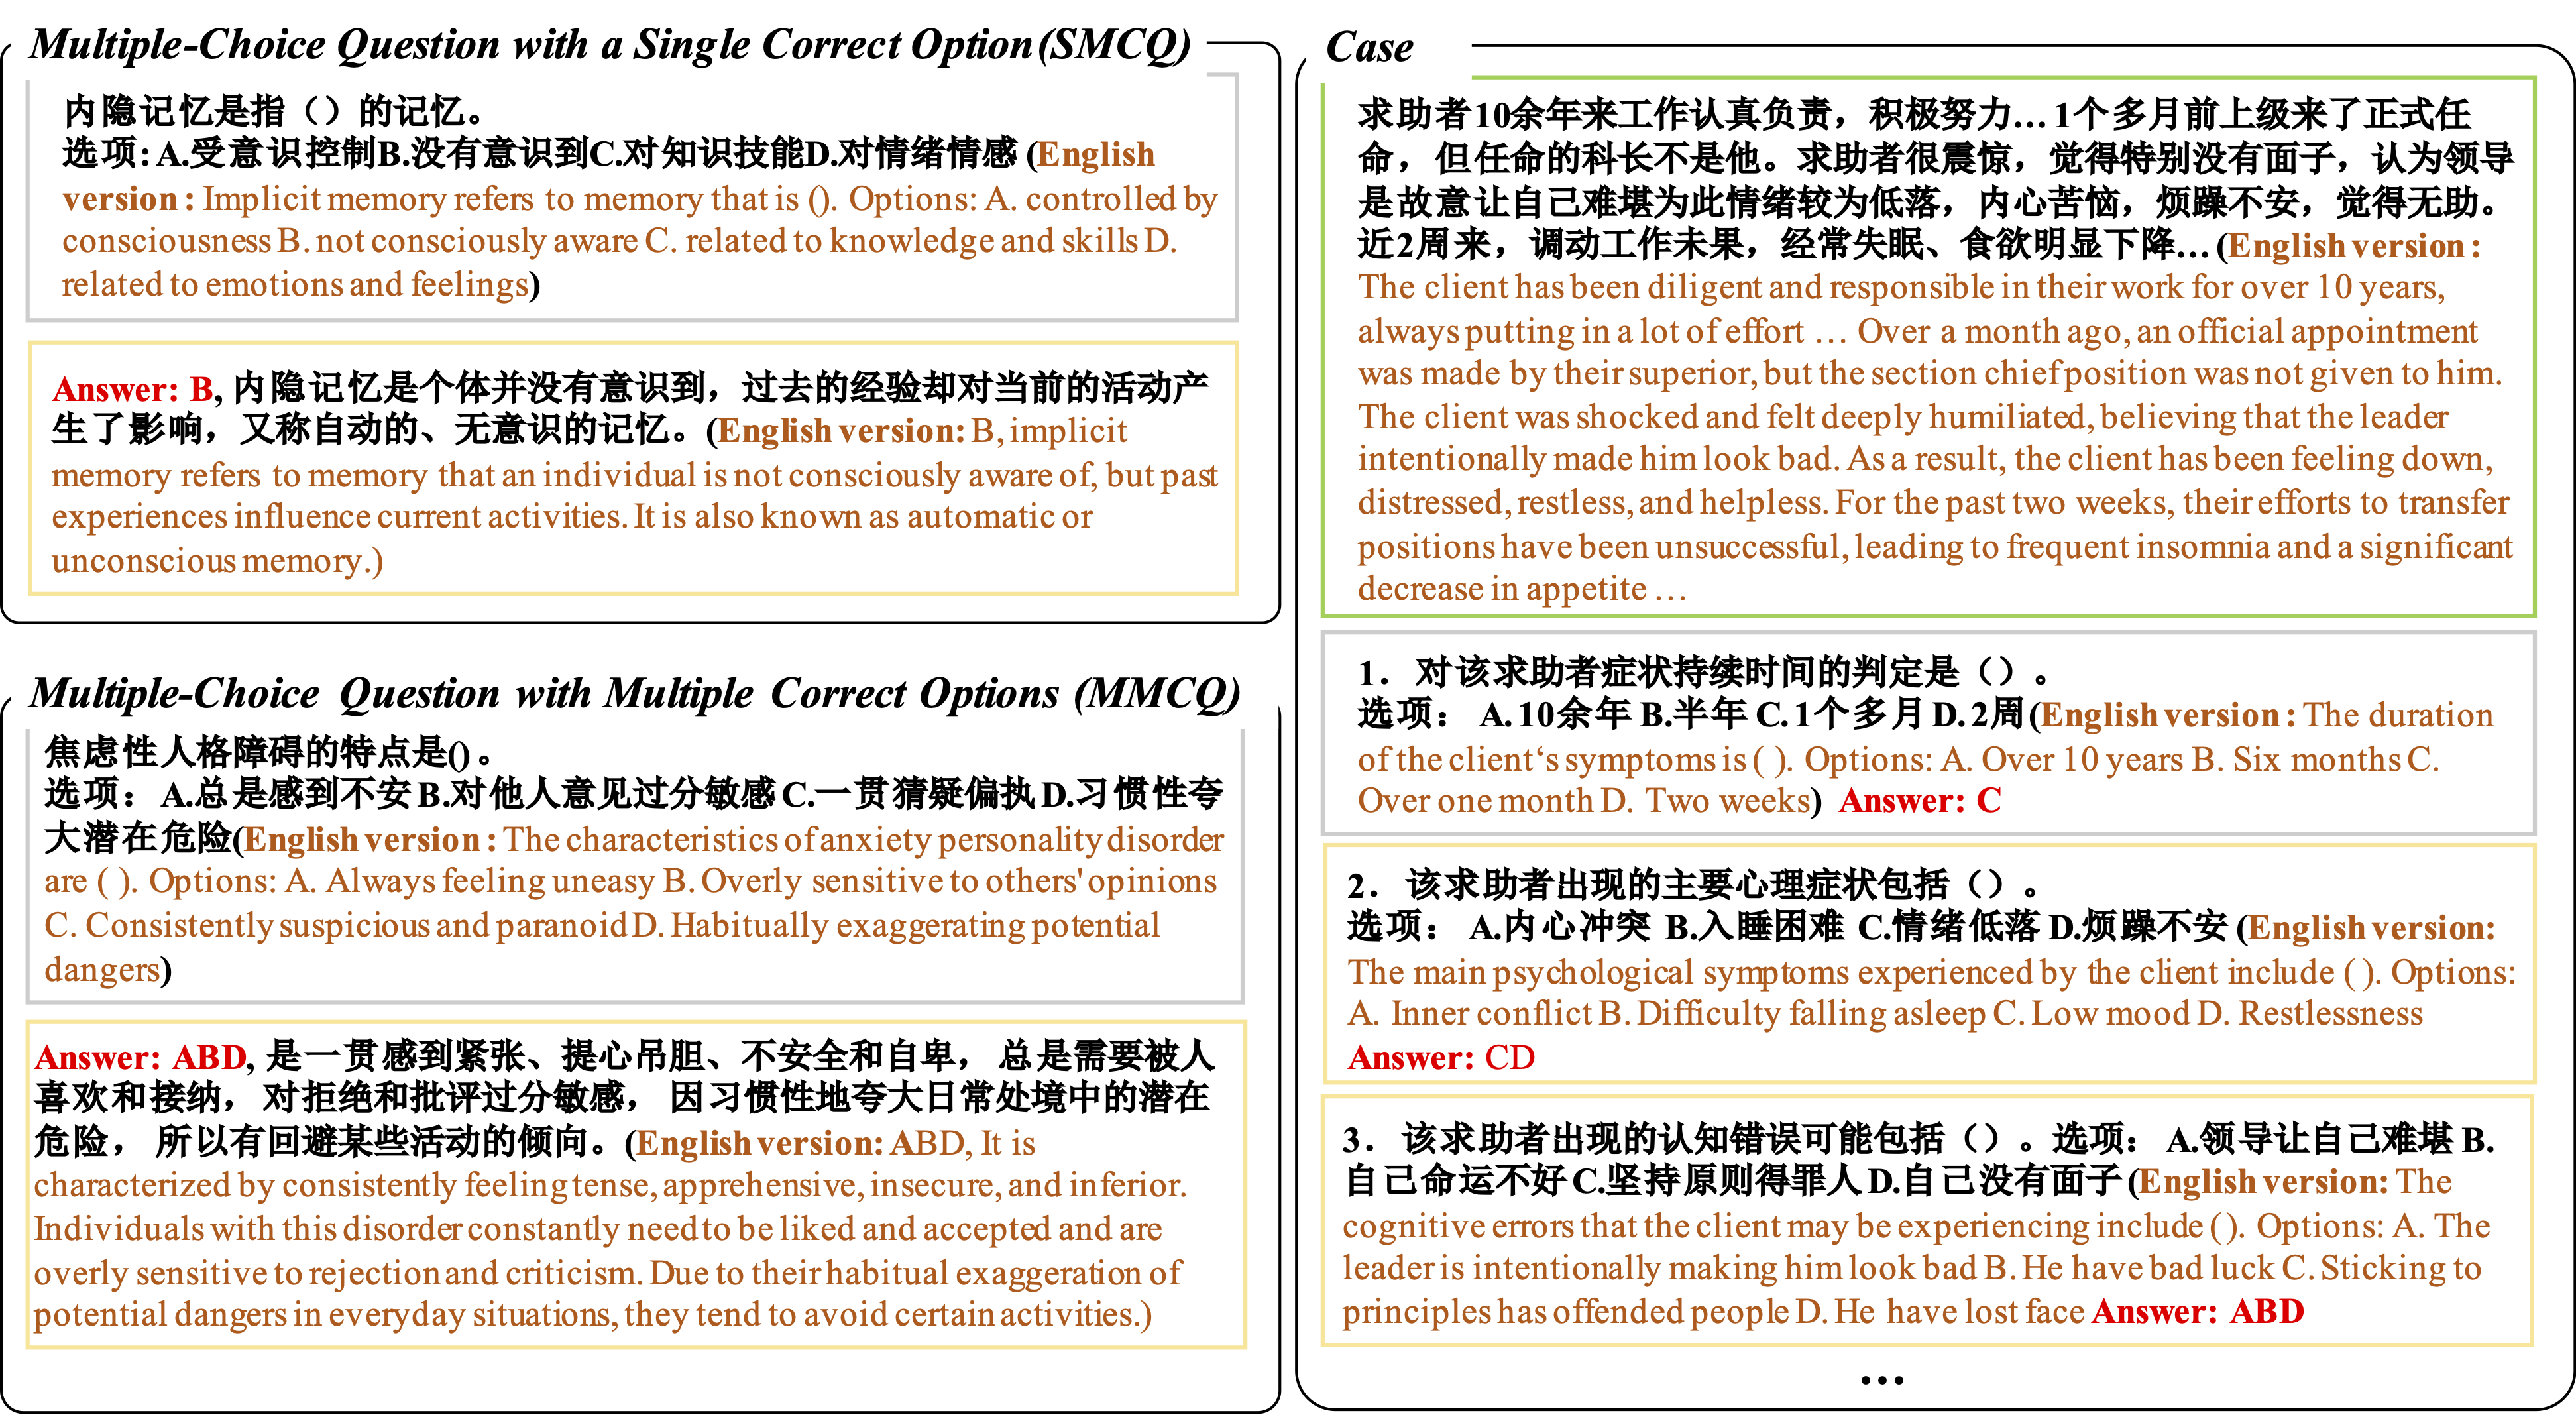
\includegraphics[width=1\textwidth]{evaluation.png}
  \caption{多项选择题示例}
  \label{fig:evaluation}
\end{figure}

评估数据集的内容可以进一步划分为以下三个部分:职业伦理、理论知识和案例分析。职业伦理部分:主要涵盖诚实守信、职业责任和社会责任等一般性原则,考察心理咨询师的道德规范和职业操守。理论知识部分:重点涉及心理学领域的基础理论与概念,包括认知心理学、发展心理学等核心知识内容。职业伦理和理论知识部分均由客观题(MCQs)组成,旨在评估受测对象对心理学领域知识的掌握程度。案例分析部分:该部分包含多项选择题与基于案例的迭代问答两种形式,旨在更好地评估模型在实际场景中的表现能力。多项选择题侧重于对案例相关专业知识的理解与应用,而基于案例的问答部分则提供了一个更加开放的评估维度,重点考察模型在实际应用中的灵活性与实用性。

经过数据收集与处理,最终得到包含 3863 道客观题(MCQs) 和 20 个案例(共计100组问答) 的评估测试数据集。客观题示例如图 ~\ref{fig:evaluation} 所示,案例问答示例如图 ~\ref{fig:case} 所示。评估测试数据的详细统计结果如表 ~\ref{benchmark-statistics} 所示,具体展示了各类问题在不同类别中的分布情况。

\begin{table}[h]
  \centering
  \caption{评估测试数据集统计}
  \label{benchmark-statistics}
  \begin{tabular}{c|cc|cc|ccc}
      \toprule
      类目 & \multicolumn{2}{c|}{\textbf{职业伦理}} & \multicolumn{2}{c|}{\textbf{理论知识}} & \multicolumn{3}{c}{\textbf{案例分析}} \\
      & \textbf{SMCQ} & \textbf{MMCQ} & \textbf{SMCQ} & \textbf{MMCQ} & \textbf{SMCQ} & \textbf{MMCQ} & \textbf{QA} \\
      \midrule
      \textbf{LEVEL 2} & 48 & 48 & 337 & 228 & 245 & 214 & 44 \\
      \textbf{LEVEL 3} & 72 & 72 & 566 & 363 & 338 & 455 & 40 \\
      \textbf{OTHERS} & 32 & 38 & 241 & 192 & 165 & 209 & 16 \\
      \midrule
      \textbf{TOTAL} & 152 & 158 & 1144 & 783 & 748 & 878 & 100 \\
      \bottomrule
  \end{tabular}
\end{table}


值得注意的是,这些问题主要被分为三级心理咨询师考试、二级心理咨询师考试和其他三大类别。根据心理学官方定义,二级心理咨询师考试的难度明显高于三级考试,这进一步确保了测试集的全面性与分级评估标准的合理性。通过以上数据的收集与预处理过程,本文构建了一个高质量、结构清晰的心理学评估测试集,为模型性能评估提供了扎实可靠的基础。

\begin{figure}[ht]
  \centering
  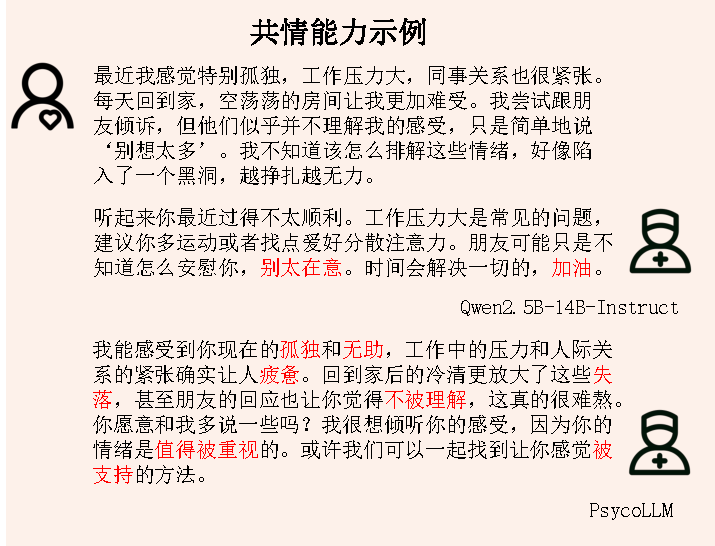
\includegraphics[width=1\textwidth]{empathy.pdf}
  \caption{共情能力示例}
  \label{fig:empathy}
\end{figure}

\begin{figure}[ht]
  \centering
  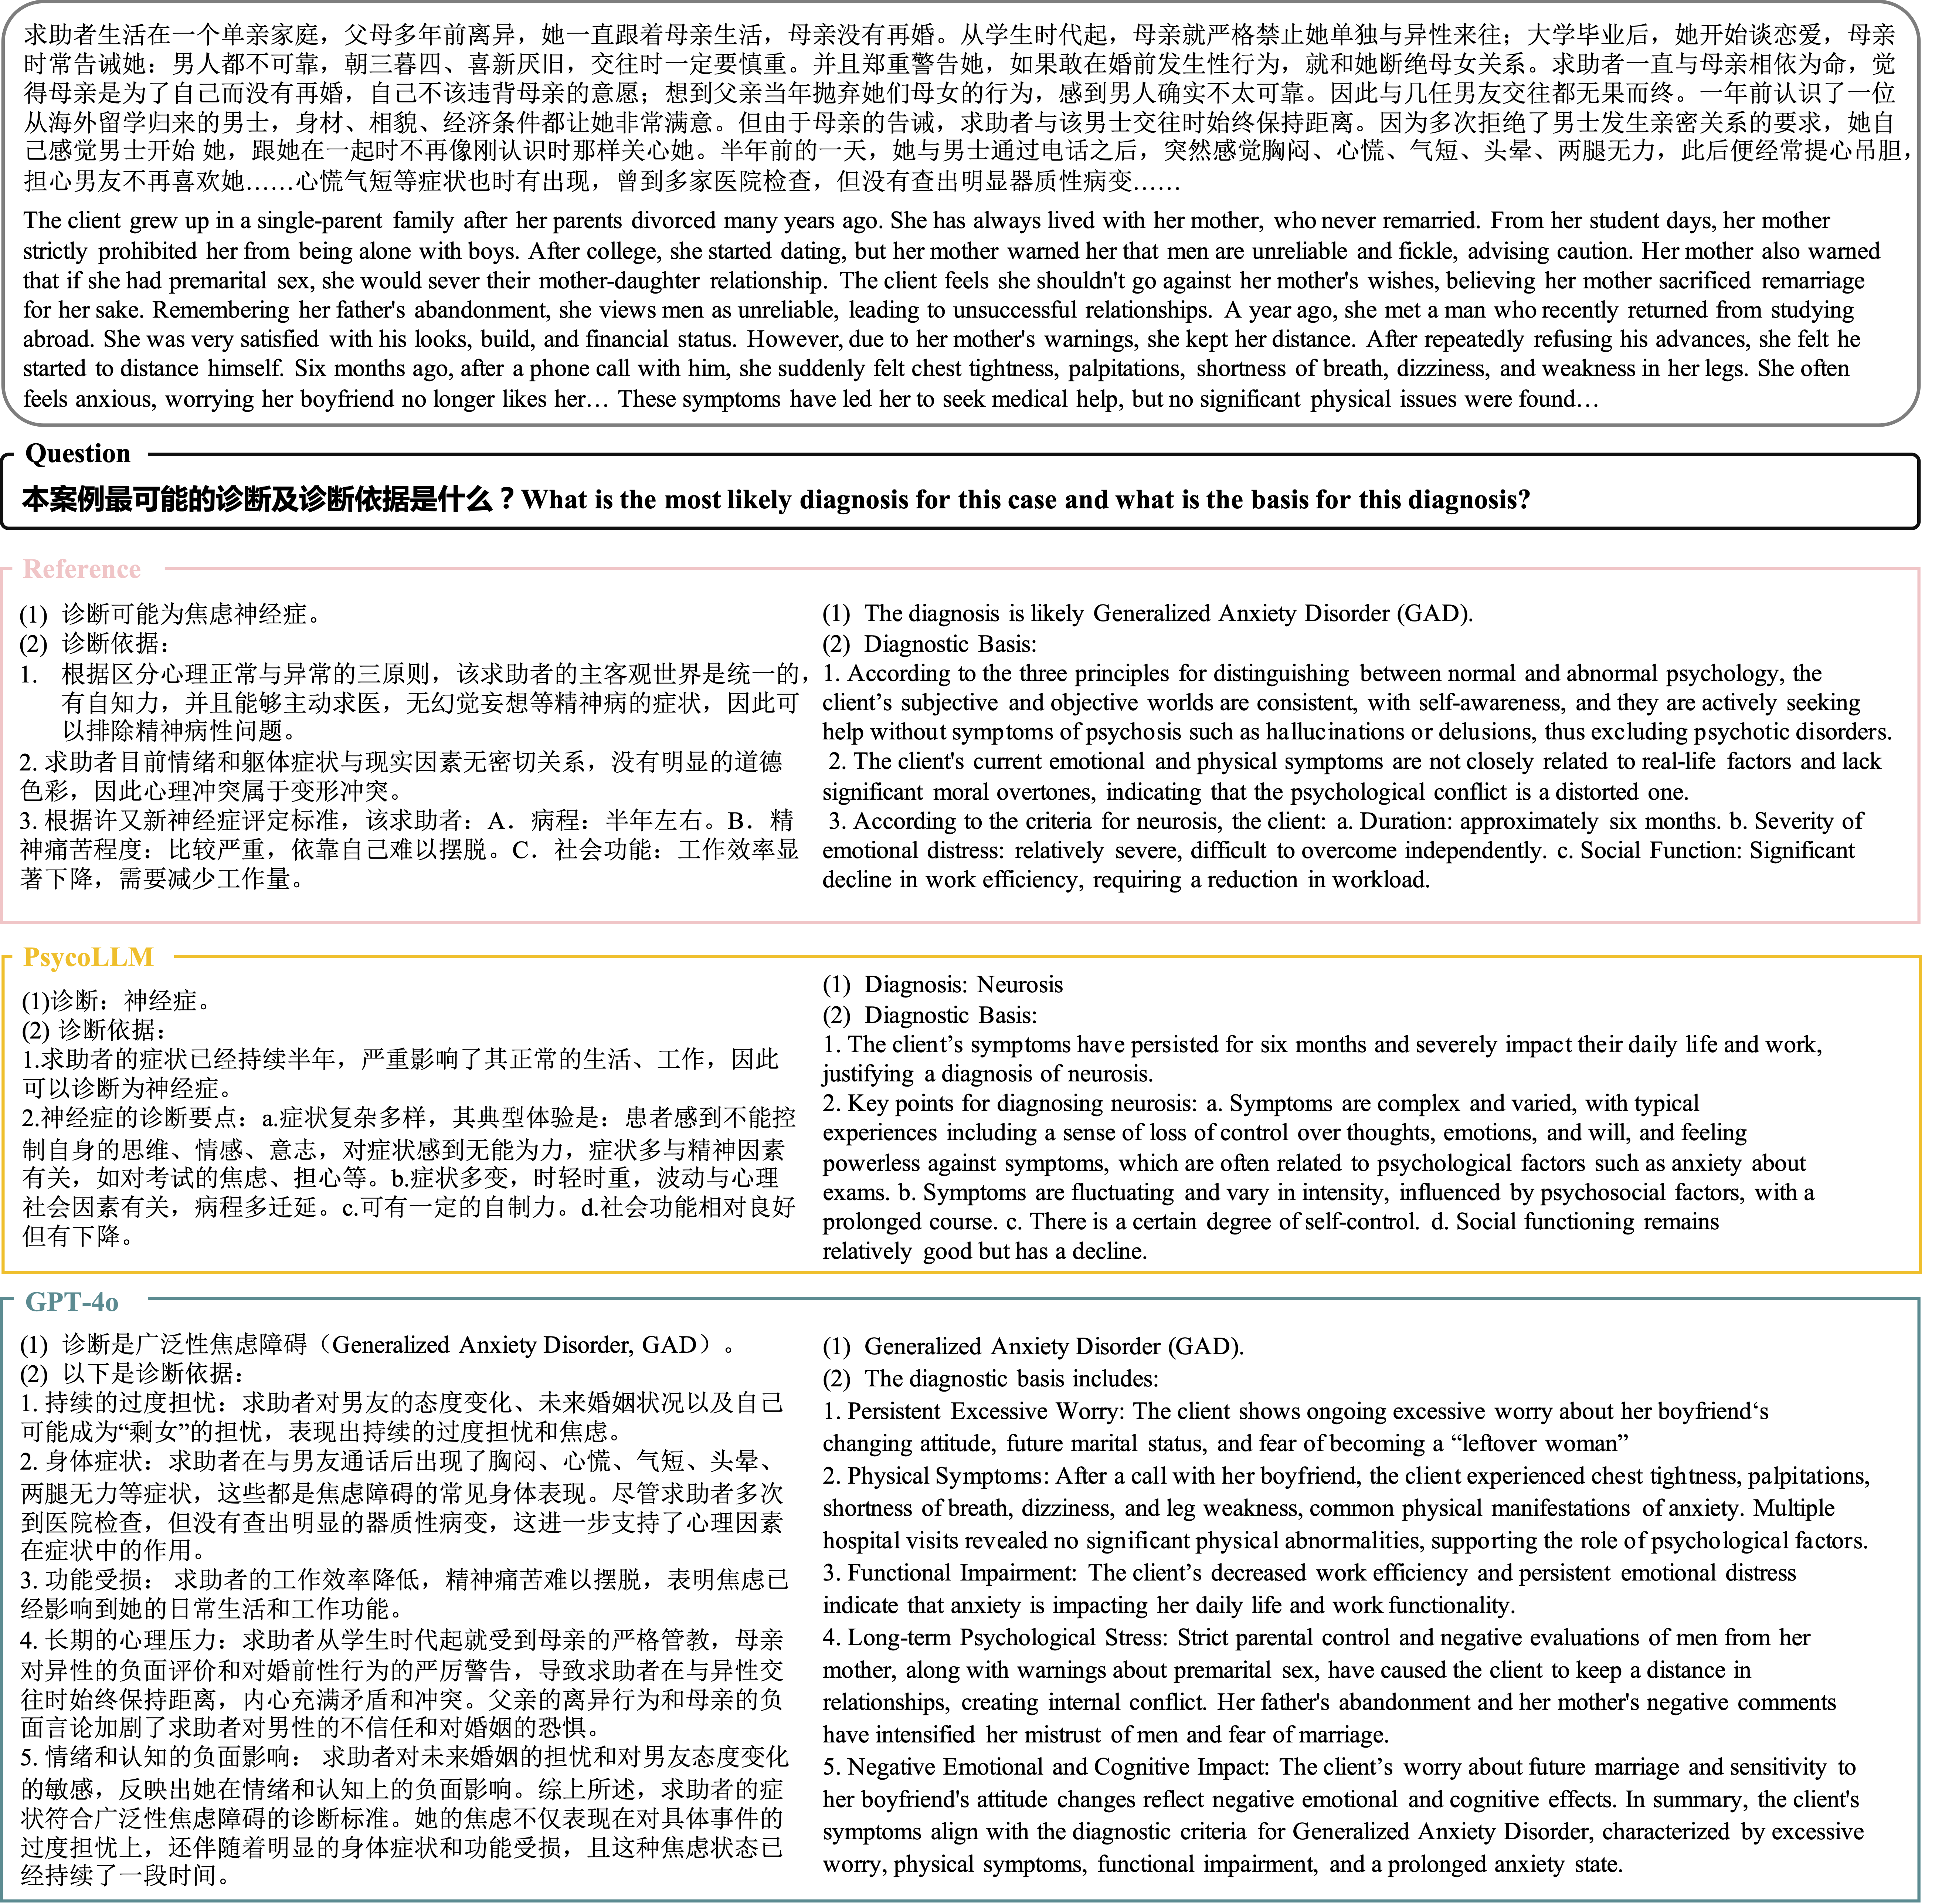
\includegraphics[width=1\textwidth]{case.png}
  \caption{案例分析示例}
  \label{fig:case}
\end{figure}

\subsection{实验设置与评价指标}

\subsubsection{实验环境设置}

本章提出的 PsycoLLM 模型使用 PyTorch 深度学习框架以及 Huggingface Transformers 框架实现,基于 LLama Factory 训练框架对模型进行训练与微调。LLama Factory 是一个高效且易于扩展的训练框架,支持大规模分布式训练,特别适用于各种架构的大模型开发。具体的硬件配置和软件配置如表 ~\ref{tab:work1-实验环境配置} 所示。

\begin{table}
  \centering
  \caption{PsycoLLM 实验环境配置}
  \label{tab:work1-实验环境配置}
  \begin{tabular}{cc}
    \toprule
    配置项 & 版本信息 \\
    \midrule
    CPU & Intel(R) Xeon(R) Gold 6326 CPU @ 2.90GHz \\
    GPU & 8 卡 NVIDIA A800 Tensor Core GPU \\
    操作系统 & Ubuntu 22.04 LTS \\
    CUDA 版本 & 12.4 \\
    Python & 3.11.9 \\
    PyTorch & 2.4.0 \\
    Huggingface Transformers & 4.46.1 \\
    \bottomrule
  \end{tabular}
\end{table}

\subsubsection{评价指标}

为了全面评估模型在心理学领域的表现,本文设计了一套系统的评估指标,适用于案例分析与多项选择题(MCQ)两类任务。

\textbf{1. 案例分析的评估指标}

在案例分析任务中,每个实例包含三个要素:$\mathcal{B}$:对给定案例的描述,包括求助者的背景、环境等信息;$\mathcal{Q}$:根据案例提出的问题,例如诊断、原因分析和治疗方案;$\mathcal{A}$:针对问题的标准参考答案。模型根据输入的 $\mathcal{B}$ 和 $\mathcal{Q}$ 生成回答 $\mathcal{O}$。本文通过文本生成任务的标准评估指标,对生成的 $\mathcal{O}$ 进行评估,具体包括:(1)ROUGE-1,评估模型输出与参考答案之间的单词重叠情况;(2)ROUGE-L,基于模型输出与参考摘要之间的最长公共子序列(LCS)匹配,衡量生成内容对关键信息的覆盖程度;(3)BLEU-4,计算4-gram(四个连续的词)重叠的精确度,用来更全面地评估机器翻译的质量;(4)BERTScore,基于预训练的 BERT 模型,通过计算生成文本和参考文本之间的余弦相似度,评估两者之间的语义相似性;(5)EmpathyNum,基于 GPT-4o 模型对文本内容进行结构化共情词汇提取,统计共情词汇数量,评估模型的共情能力。

\textbf{2. 多项选择题(MCQ)的评估指标}

对于单选题(SMCQ),本文使用标准准确率作为评估指标,计算模型预测完全正确的答案占总问题数量的比例,反映模型的精确度。对于多选题(MMCQ),本文引入两种评估指标:标准准确率:定义为完全正确答案的比例,仅统计所有选项均正确的回答。弹性准确率(Elastic Accuracy):该指标考虑完全正确和部分正确的回答,允许部分答案中包含正确选项但不包含错误选项。弹性准确率的计算公式如下:
\begin{equation}
  \text{Elastic accuracy} = \frac{|\text{predicted answer}|}{|\text{correct answer}|},
\end{equation}
其中,$|\cdot|$ 表示答案中选项的数量。弹性准确率为模型提供了一种更加灵活的评估方式,能够识别出大部分正确但不完全精确的回答,体现模型在实际任务中的表现能力。通过上述指标,案例分析侧重于模型生成文本的质量和流畅性,而多项选择题侧重于模型对知识点的精确掌握与实际应用能力。这套评估体系确保了对心理健康大模型性能的全面分析与验证。

\subsection{对比实验结果与分析}

\subsubsection{基线设置}

为了验证本章提出的 PsycoLLM 模型在心理学领域的有效性,本文进行了一系列对比实验,本章当下主流的通用领域大模型和心理情感相关大模型作为基线对比模型,各个基线模型的详细介绍如下所示:

\textbf{1. 通用语言大模型}

% GPT-4o:由 OpenAI 训练的多语言、多模态 GPT 大语言模型,在语音、多语言和视觉基准测试中取得了最先进的性能。

% Qwen2.5 系列模型:包括 Qwen2.5-7B-Instruct 和 Qwen2.5-14B-Instruct, 由阿里云通义实验室开发,采用 SwiGLU 激活函数、RoPE 位置编码和多头注意力机制进行预训练,语料总量超过 3 万亿 token。这些模型在中文语言任务上表现出色。

% InternLM2.5 系列模型:包括 InternLM2.5-7B-Chat 和 InternLM2.5-20B-Chat 版本,由上海人工智能实验室研发。该系列模型在多轮对话和复杂推理任务上表现优异,但未经过心理学数据的专门优化。

% Deepseek 系列模型:包括 Deepseek-LLM-7B-Chat 和 Deepseek-MoE-16B-Chat,由 Deepseek AI 团队开发。这些模型在多任务自然语言处理任务中取得了较好效果,是综合性强的基线模型。

% LLaMA3-Chinese-8B-Chat 模型:基于 Meta 公司的 LLaMA3 模型,由 LLaMA 中文社区通过中文指令数据集进行微调优化训练的大模型。

% GLM-4-9B 模型:清华大学知识工程组与智谱 AI 联合发布的对话生成模型,专注于中文生成任务。
不同研究机构和企业推出了多种具备强大语言理解与生成能力的模型。以下是几种具有代表性的大语言模型:(1)GPT-4o:由 OpenAI 训练的多语言、多模态大语言模型,在语音、多语言和视觉等多个基准测试中取得了最先进的性能,展现出卓越的综合能力。(2)Qwen2.5 系列模型:由 阿里云通义实验室 开发,包括 Qwen2.5-7B-Instruct 和 Qwen2.5-14B-Instruct。该系列模型采用 SwiGLU 激活函数、RoPE 位置编码及多头注意力机制进行预训练,语料总量超过 3 万亿 tokens,在中文语言任务中表现尤为突出。(3)InternLM2.5 系列模型:由 上海人工智能实验室 研发,涵盖 InternLM2.5-7B-Chat 和 InternLM2.5-20B-Chat 两个版本,该系列在多轮对话和复杂推理任务上表现优异,但未经过专门的心理学数据优化,在心理健康相关任务上的泛化能力仍有待提升。(4)Deepseek 系列模型:由 Deepseek AI 团队 开发,包括 Deepseek-LLM-7B-Chat 和 Deepseek-MoE-16B-Chat。该系列模型在多任务自然语言处理(NLP)任务中取得了良好效果,具备较强的综合性,常被作为对比实验中的基线模型。(5)LLaMA3-Chinese-8B-Chat:基于 Meta 公司的 LLaMA3 模型,由 LLaMA 中文社区通过中文指令数据集进行微调训练,优化了其在中文任务上的性能。(6)GLM-4-9B:由清华大学知识工程组与智谱 AI 联合发布的对话生成模型,专注于中文生成任务,在文本生成质量与语言理解方面均表现出色。

\textbf{2. 心理领域模型}

目前主要的心理领域模型包括以下两类:(1)MindChat 系列模型:该系列模型基于 Qwen2-7B-Instruct 和 Qwen2-14B-Instruct 进行微调,专门针对心理健康对话场景优化。通过引入心理健康多轮对话数据集进行训练,MindChat 具备更强的情境理解能力和共情对话能力,能够在心理咨询任务中提供更自然、连贯且专业的对话支持。该系列模型包括 MindChat-Qwen2-7B 和 MindChat-Qwen2-14B,分别适用于不同计算资源需求的应用场景。(2)EmoLLM 模型:该模型基于 InternLM2.5-7B-Chat 进行全量微调,主要通过情感对话数据集优化训练,以增强其情绪感知和情感生成能力。EmoLLM 旨在生成更符合情感语境的文本,使其在心理支持、情绪疏导和人机交互等任务中具备更强的共情能力和自然对话流畅度。

\subsubsection{结果分析}

(1)客观评估结果

为了探索不同模型在心理健康评估测试中的表现,本文对客观题目进行了评估,结果见表 \ref{tab:work1-客观题目评估结果}。SMCQ 和 MMCQ 分别是标准准确率结果,MMCQ-E 为 MMCQ 的弹性准确率结果, AVG 为平均准确率,AVG-E 为平均弹性准确率。以下是从结果中总结出的分析:

\begin{table}[h]
    \centering
    \caption{客观题目评估结果}
    \resizebox{1\textwidth}{!}{
    \label{tab:work1-客观题目评估结果}
    \begin{tabular}{c|ccc|ccc|ccc|cc}
        \toprule
        模型 & \multicolumn{3}{c|}{职业伦理} & \multicolumn{3}{c|}{理论知识} & \multicolumn{3}{c|}{案例分析} & \multicolumn{2}{c}{平均准确率} \\
        & SMCQ & MMCQ & MMCQ-E & SMCQ & MMCQ & MMCQ-E & SMCQ & MMCQ & MMCQ-E & AVG & AVG-E \\
        \midrule
        LLaMA3-Chinese-8B-Chat & 42.10 & 18.35 & 25.84 & 29.54 & 13.64 & 18.68 & 21.39 & 10.70 & 21.92 & 22.62 & 26.57 \\
        Deepseek-LLM-7B-Chat & 63.82 & 40.97 & 52.29 & 46.44 & 25.23 & 36.98 & 38.09 & 16.32 & 29.64 & 38.87 & 45.09 \\
        InternLM2.5-7B-Chat & 71.07 & 40.52 & 54.81 & 63.75 & 26.29 & 41.65 & 44.53 & 18.92 & 27.99 & 44.17 & 50.64 \\
        GLM-4-9B & 79.82 & 54.17 & 64.50 & 61.92 & 27.35 & 43.25 & 40.82 & 20.14 & 39.53 & 47.20 & 54.97 \\
        Qwen2.5-7B-Instruct & 79.39 & 55.47 & 66.98 & 62.76 & 28.45 & 44.61 & 40.92 & 21.47 & 41.29 & 47.69 & 55.63 \\
        Deepseek-MOE-16B-Chat & 81.92 & 57.13 & 68.09 & 61.89 & 28.92 & 45.79 & 43.20 & 22.13 & 40.63 & 48.67 & 57.36 \\
        InternLM2.5-20B-Chat & 83.21 & 58.29 & 69.43 & 63.92 & 29.41 & 46.12 & 44.09 & 22.67 & 41.29 & 49.74 & 58.28 \\
        Qwen2.5-14B-Instruct & 84.13 & 59.12 & 70.29 & 64.67 & 30.54 & 46.97 & 44.23 & 23.60 & 41.90 & 50.32 & 58.71 \\
        GPT-4o & 88.15 & 45.57 & 68.79 & \textbf{74.65} & 24.10 & 45.07 & \textbf{65.53} & 13.67 & 34.53 & 52.94 & 60.45 \\
        \midrule
        MindChat & 55.26 & 13.29 & 30.13 & 33.94 & 7.55 & 23.35 & 9.65 & 4.78 & 12.09 & 20.74 & 27.40  \\
        EmoLLM & 55.26 & 20.25 & 33.06 & 38.54 & 12.75 & 24.40 & 24.59 & 11.88 & 22.28 & 27.21 & 33.02 \\
        \midrule
        PsycoLLM & \textbf{89.96} & \textbf{70.89} & \textbf{75.32} & 73.78 & \textbf{49.34} & \textbf{55.43 }& 56.93 & \textbf{35.24} & \textbf{43.57} & \textbf{62.89} & \textbf{65.70} \\
        \bottomrule
    \end{tabular}
    }
\end{table}

第一,相比于理论知识部分,模型在职业伦理部分表现更为优异。这可能是因为职业伦理相关内容与通用领域数据集的匹配度更高,而这些数据通常包含大量与伦理相关的内容,使得通用语言大模型在伦理评估中表现较强。而理论知识的学习则需要更为专门化的数据,这在通用领域训练中出现的比例较少。

第二,在选择题(MCQs)中,多选题(MMCQs)的准确率明显低于单选题(SMCQs)。这种差异可能是由于多选题在确保全面性和准确性时难度更大,模型需要同时选择多个正确选项,增加了回答的复杂性,从而影响了整体准确率。

第三,GPT-4o 在理论知识和案例分析的单选题中表现最佳。这表明,尽管该模型是为通用领域训练的,但其强大的通用能力为有效解决心理健康领域的特定任务提供了坚实的基础,包括心理学概念和基于案例的评估。

第四,多款模型表现出通过评估测试中多选题的能力,这些题目主要源自权威心理咨询考试。其中,只有本文的模型在标准准确率(Standard Accuracy)上平均超过了 60\%。在弹性准确率(Elastic Accuracy)方面,GPT-4o 和本文 PsycoLLM 模型的平均分均超过了 60\%。这一结果突显了大语言模型在心理健康领域提供辅助支持的潜力。

第五,本文提出的模型在标准准确率方面相较其他模型有显著提高,特别是在心理健康领域任务的性能上。这验证了本文提出的心理数据集在提升模型性能方面的有效性。

(2)基于案例问答的结果

本文对主观问题的评估结果见表 \ref{tab:work1-案例分析主观评估结果},在自动评估中,使用 ROUGE 和 BLEU 等指标的得分相对较低。这可能是因为这些指标难以捕捉自然语言生成中的语义等价性与上下文适切性,而更多关注的是表面级的 n-gram 匹配。因此,本文将 BERTScore 纳入评估框架中。大多数模型在 BERTScore 指标上得分稳定在 63 到 65 之间,显示出 BERTScore 的一致性和可靠性。本文模型在 R-1、B-4 和 BERTScore 上表现优异,而 EmoLLM 在 R-L 指标上表现较好。此外,尽管 EmoLLM 和 MindChat 在选择题中的表现一般,但它们在 R-1、R-L 和 B-4 上表现相对较强。这可能是因为这些模型使用了心理对话数据进行微调,使其在案例信息的理解和高质量回复的生成上具备优势。通过观察 EmpathyNum 指标,本文的模型在生成的共情词汇数量上也更多。如图 ~\ref{fig:empathy} 所示,本文模型相比 Qwen2.5-14B-Instruct 的共情能力也更强。通过对本文模型和 GPT-4o 的案例生成结果进行对比(如图 \ref{fig:case} 所示),可以发现,两者都能有效识别患者的大部分问题,但生成的答案风格有所不同:GPT-4o 更倾向于提供详细、具体的回答,而本文模型则以简洁的回答为主。

\begin{table}
  \centering
  \caption{案例分析主观评估结果}
  \label{tab:work1-案例分析主观评估结果}
  \begin{tabular}{cccccc}
    \toprule
    模型 & ROUGE-1 & ROUGE-L & BLEU-4 & BERTScore & EmpathyNum \\
    \midrule
    LLaMA3-Chinese-8B-Chat & 23.11 & 17.28 & 1.25 & 62.18 & 84 \\
    Deepseek-LLM-7B-Chat & 22.01 & 14.13 & 1.83 & 64.43 & 153 \\
    InternLM2.5-7B-Chat & 24.07 & 17.76 & 1.92 & 64.26 & 158 \\
    GLM-4-9B & 22.93 & 14.20 & 15.59 & 64.86 & 187 \\
    Qwen2.5-7B-Instruct & 22.65 & 13.47 & 1.50 & 64.76 & 167 \\
    Deepseek-MOE-16B-Chat & 22.87 & 14.05 & 1.63 & 64.92 & 192 \\
    InternLM2.5-20B-Chat & 23.12 & 14.23 & 1.68 & 64.98 & 209 \\
    Qwen2.5-14B-Instruct & 23.45 & 14.56 & 1.73 & 65.12 & 334 \\
    GPT-4o & 23.67 & 14.78 & 1.78 & 65.23 & 329 \\
    \midrule
    MindChat & 24.34 & 17.49 & 1.71 & 63.59 & 179 \\
    EmoLLM & 23.34 & \textbf{17.98} & 1.94 & 63.41 & 276 \\
    \midrule
    PsycoLLM & \textbf{25.12} & 17.67 & \textbf{2.08} & \textbf{65.76} & \textbf{386} \\
    \bottomrule
  \end{tabular}
\end{table}


(3)难度对性能的影响

本文进一步在二级心理咨询师考试和三级心理咨询师考试中对 PsycoLLM、Qwen2.5-14B-Instruct 的表现进行了比较,结果见表 \ref{tab:work1-不同模型在二级和三级心理咨询师考试中的表现}。从结果来看,在理论知识部分,模型在三级考试中的表现普遍优于二级考试。这一差异可能是由于二级考试要求对心理学概念有更广泛的理解,并对相关理论框架有更深入的掌握。然而,在职业伦理和案例分析部分,模型在二级考试中的表现优于三级考试。这表明,在某些情况下,大语言模型对难度的感知可能与人类不同。并非所有被人类认为复杂的部分对模型来说都具有挑战性。

\begin{table}[h]
    \centering
    \caption{不同模型在二级和三级心理咨询师考试中的表现}
    \resizebox{1\textwidth}{!}{
    \label{tab:work1-不同模型在二级和三级心理咨询师考试中的表现}
    \begin{tabular}{c|c|ccc|ccc|ccc}
        \toprule
        模型 & 类目 & \multicolumn{3}{c|}{职业伦理} & \multicolumn{3}{c|}{理论知识} & \multicolumn{3}{c}{案例分析} \\
        & & SMCQ & MMCQ & MMCQ-E & SMCQ & MMCQ & MMCQ-E & SMCQ & MMCQ & MMCQ-E \\
        \midrule
        Qwen2.5-14B-Instruct & LEVEL 2 & 83.34 & 62.50 & 70.65 & 67.35 & 30.26 & 48.83 & 43.26 & 22.89 & 40.38 \\
        Qwen2.5-14B-Instruct & LEVEL 3 & 76.39 & 51.39 & 62.27 & 69.38 & 27.82 & 47.02 & 36.79 & 19.12 & 40.54 \\
        \midrule
        PsycoLLM & LEVEL 2 & 90.91 & 72.92 & 77.08 & 70.15 & 47.14 & 51.91 & 57.55 & 33.64 & 41.39 \\
        PsycoLLM & LEVEL 3 & 87.50 & 68.06 & 72.11 & 74.73 & 51.10 & 56.91 & 50.71 & 36.70 & 44.57 \\
        \bottomrule
    \end{tabular}
    }
\end{table}

(4)心理健康微调对通用能力的影响

为了评估在心理数据集上进行微调对模型通用推理能力的影响,本文比较了 PsycoLLM 与其未微调的评估模型 Qwen2.5-14B-Instruct 的表现。实验涵盖多个广泛使用的通用评估,包括 MMLU、CMMLU、GSM8K 和 CEVAL,MMLU、CMM、CEVAL 使用 5-shot 进行评估,GSM8K 使用 8-shot 进行评估,结果见表 \ref{tab:work1-模型在通用评估测试中的表现}。结果显示,本文模型在这些通用任务中的表现与基准模型相当,甚至在 GSM8K 基准上表现更好。这表明,针对心理数据集的微调并未显著削弱模型的通用推理能力。然而,在某些基准测试(如 MMLU、CMMLU 和 CEVAL)中,本文模型 的表现略有下降。这反映了在领域特定微调与通用能力之间平衡的必要性。这种下降可能是因为微调过程中某些通用任务未被充分考虑,或者存在过拟合心理数据集的风险,从而导致对通用任务的鲁棒性降低。

\begin{table}
  \centering
  \caption{模型在通用评估测试中的表现}
  \label{tab:work1-模型在通用评估测试中的表现}
  \begin{tabular}{ccccc}
    \toprule
    模型 & MMLU & CMMLU & GSM8K & CEVAL \\
    \midrule
    Qwen2.5-14B-Instruct & 66.29 & 76.43 & 69.32 & 76.08 \\
    PsycoLLM & 65.92 & 74.93 & 73.48 & 75.26 \\
    \bottomrule
  \end{tabular}
\end{table}

(5)讨论

模型规模的影响:在同一模型系列中,参数规模较大的模型通常表现更优。例如,Qwen2.5-14B-Instruct 和 InternLM2.5-20B-Chat 相较于其较小的版本(如 Qwen2.5-7B-Instruct 和 InternLM2.5-7B-Chat)表现更好。这种提升归因于更大的模型容量能够捕捉更复杂的模式并有效学习数据中的文本表示。然而,不同模型系列之间的对比结果存在差异。例如,Qwen2.5-14B-Instruct 在多选题评估中优于 InternLM2.5-20B-Chat 和 Deepseek-MOE-16B-Chat。这表明除了模型规模外,训练语料和训练过程等因素对性能也有重要影响。

多选题中的模型偏好:实验发现,不同模型在多选题上的响应模式存在显著差异。例如,GPT-4o 更倾向于仅选择单一选项,而 Qwen2.5-14B-Instruct 则倾向于选择所有选项。这种行为导致 GPT-4o 在从标准准确率切换到弹性准确率时获得较大提升。这种差异可能与训练数据有关。GPT-4o 的训练数据主要为英文语料,而英文语境中多选题相对较少,因此模型在应对多选题时可能缺乏经验。

微调模型与通用模型:在所有模型中,EmoLLM 和 MindChat 使用心理相关数据集进行微调,这使得它们在基于案例的问答任务中相较于通用模型表现更优。然而,由于知识类数据的融入不足,其在选择题评估中的表现较为一般。这表明微调过程中的数据选择对模型性能有显著影响。

\section{本章小结}

本章通过详细的实验设计与结果分析,全面评估了本文提出的多模态情感描述大模型在心理健康领域的表现。通过与多种通用语言模型及心理健康相关模型的对比实验,结果表明本文模型在单选题和多选题的情绪识别任务中表现突出,特别是在心理健康基准测试中的标准准确率显著提升。同时,基于案例的问答实验进一步验证了模型在生成情绪一致性和语义连贯性上的优势。此外,通过难度实验和心理微调对通用能力的影响分析,探讨了领域特定微调与通用能力之间的平衡问题。综合来看,实验结果充分证明了本文提出的心理健康领域数据集和大模型方法在提升任务性能与适用性方面的有效性。
